%============================================================================
% tento soubor pouzijte jako zaklad
% (c) 2008 Michal Bidlo
% E-mail: bidlom AT fit vutbr cz
%============================================================================
% kodovaní: iso-8859-2 (zmena prikazem iconv, recode nebo cstocs)
%----------------------------------------------------------------------------
% zpracování: make, make pdf, make desky, make clean
% připomínky posílejte na e-mail: bidlom AT fit.vutbr.cz
% vim: set syntax=tex encoding=latin2:
%============================================================================
%\documentclass[cover]{fitthesis} % odevzdani do wisu - odkazy, na ktere se da klikat
%\documentclass[cover,print]{fitthesis} % pro tisk - na odkazy se neda klikat
%\documentclass[english,print]{fitthesis} % pro tisk - na odkazy se neda klikat
%      \documentclass[english]{fitthesis}
% * Je-li prace psana v anglickem jazyce, je zapotrebi u tridy pouzit 
%   parametr english nasledovne:
\documentclass[english]{fitthesis}
%\documentclass[english,print]{fitthesis}
%\documentclass[english, cover]{fitthesis}
% * Neprejete-li si vysazet na prvni strane dokumentu desky, zruste 
%   parametr cover
% zde zvolime kodovani, ve kterem je napsan text prace
% "latin2" pro iso8859-2 nebo "cp1250" pro windows-1250, "utf8" pro "utf-8"
%\usepackage{ucs}
%\usepackage[latin2]{inputenc}
\usepackage[utf8]{inputenc}
\usepackage[T1, IL2]{fontenc}
\usepackage{url}
\DeclareUrlCommand\url{\def\UrlLeft{<}\def\UrlRight{>} \urlstyle{tt}}

%zde muzeme vlozit vlastni balicky

%\usepackage{float}
\usepackage{pdfpages}

\usepackage[colorinlistoftodos]{todonotes}
% personalised TODO boxes:
\newcommand{\todoW}[1]{\todo[inline, color=green!80]{\textbf{Write:} #1}}
\newcommand{\todoL}[1]{\todo[inline, color=cyan!80]{\textbf{Literature:} #1}}
\newcommand{\todoR}[1]{\todo[inline, color=pink!80]{\textbf{Rewrite:} #1}}
\newcommand{\todoP}[1]{\todo[inline, color=orange!80]{\textbf{Add picture:} #1}}
\newcommand{\todoO}[1]{\todo[inline, color=blue!30]{\textbf{Others:} #1}}
\newcommand{\todoF}[1]{\todo[inline, color=yellow!30]{\textbf{Reference:} #1}}

% CANCEL ALL TODOS:
%\renewcommand{\todoW}[1]{}\renewcommand{\todoL}[1]{}\renewcommand{\todoR}[1]{}\renewcommand{\todoP}[1]{}\renewcommand{\todoO}[1]{}\renewcommand{\todoF}[1]{}

\newcommand{\funcName}[1]{\path{#1}}
\newcommand{\newExpr}[1]{\emph{#1}}
\newcommand{\keyName}[1]{\textbf{#1}}

% =======================================================================
% balíček "hyperref" vytváří klikací odkazy v pdf, pokud tedy použijeme pdflatex
% problém je, že balíček hyperref musí být uveden jako poslední, takže nemůže
% být v šabloně
\ifWis
\ifx\pdfoutput\undefined % nejedeme pod pdflatexem
\else
  \usepackage{color}
  \usepackage[unicode,colorlinks,hyperindex,plainpages=false,pdftex]{hyperref}
  %\usepackage[hidelinks]{hyperref}
  \definecolor{links}{rgb}{0.4,0.5,0}
  \definecolor{anchors}{rgb}{1,0,0}
  \def\AnchorColor{anchors}
  \def\LinkColor{links}
  \def\pdfBorderAttrs{/Border [0 0 0] }  % bez okrajů kolem odkazů
  \pdfcompresslevel=9
\fi
\fi

%Informace o praci/projektu
%---------------------------------------------------------------------------
\projectinfo{
  %Prace
  project=BP,            %typ prace BP/SP/DP/DR
  year=2015,             %rok
  date=\today,           %datum odevzdani
  %Nazev prace
  title.cs={Aplikace pro sledování objektů ve videu},  %nazev prace v cestine
  title.en={Application for Video Tracking}, %nazev prace v anglictine
  %Autor
  author={Martin Borek},   %jmeno prijmeni autora
  %author.title.p=Bc., %titul pred jmenem (nepovinne)
  %author.title.a=PhD, %titul za jmenem (nepovinne)
  %Ustav
  department=UITS, % doplnte prislusnou zkratku: UPSY/UIFS/UITS/UPGM
  %Skolitel
  supervisor= Filip Orság, %jmeno prijmeni skolitele
  supervisor.title.p=Ing.,   %titul pred jmenem (nepovinne)
  supervisor.title.a={Ph.D.},    %titul za jmenem (nepovinne)
  %Klicova slova, abstrakty, prohlaseni a podekovani je mozne definovat 
  %bud pomoci nasledujicich parametru nebo pomoci vyhrazenych maker (viz dale)
  %===========================================================================
  %Klicova slova
  keywords.cs={Video Anonymizer, anonymizace, sledování objektů ve videu, úprava videa, sledování částic, QT, FFmpeg}, %klicova slova v ceskem jazyce
  keywords.en={Video Anonymizer, anonymization, video tracking, video editing, QT, FFmpeg, particle tracking}, %klicova slova v anglickem jazyce
  %Abstract
  abstract.cs={Předložená bakalářská práce pojednává o implementaci aplikace Video Anonymizer. Tato aplikace sleduje objekty ve videu a upravuje jejich vzhled. Práce se zabývá \mbox{zpracováním} videa s použitím knihovny FFmpeg, kde se zaměřuje především na vyhledávání snímků. Soustřeďuje se také na sledování více objektů, úpravu jejich trajektorií a na jejich anonymizaci; upřednostňovaný způsob anonymizace je rozmazání objektu. Dále je zde rozebráno vytváření vícejazyčného uživatelsky přívětivého grafického uživatelského rozhraní s pomocí knihovny QT. Při testování uživatelské přívětivosti tohoto grafického uživatelského rozhraní bylo zjištěno, že aplikace je snadno ovladatelná již při jejím prvním použití. Také bylo ověřeno, že uživatelská nápověda obsahuje všechny potřebné informace a je snadno dostupná přímo z aplikace.}, % abstrakt v ceskem jazyce
  abstract.en={This thesis focuses on an implementation of an application Video Anonymizer. The application tracks objects in a video and changes their appearance. The thesis deals with processing videos when using the FFmpeg library. It covers especially issues of frames seeking. It also covers tracking multiple objects, manually correcting their trajectories and anonymizing them. The preferred way of anonymization is defocusing objects. Furthermore, the thesis describes creating a multilingual user-friendly graphical user interface with the QT framework. A usability testing was performed and revealed that the graphical user interface is easy to use even when used for the first time. Besides, it proved that a user's guide is comprehensive and easily accessible right in the application.}, % abstrakt v anglickem jazyce
  %Prohlaseni
  declaration={Prohlašuji, že jsem tuto bakalářskou práci vypracoval samostatně pod vedením pana Ing. Filipa Orsága, Ph.D.},
  %Podekovani (nepovinne)
  acknowledgment={Na tomto místě bych rád poděkoval vedoucímu mé práce panu Ing. Filipu Orságovi, Ph.D. za zajímavé téma, trpělivost a věnovaný čas. Také bych chtěl velmi poděkovat rodičům, celé mé rodině i přátelům za podporu během studia i psaní této práce.} % nepovinne
}

%Abstrakt (cesky, anglicky)
%\abstract[cs]{Do tohoto odstavce bude zapsán výtah (abstrakt) práce v českém jazyce.}
%\abstract[en]{Do tohoto odstavce bude zapsán výtah (abstrakt) práce v anglickém jazyce.}

%Klicova slova (cesky, anglicky)
%\keywords[cs]{Sem budou zapsána jednotlivá klíčová slova v českém jazyce, oddělená čárkami.}
%\keywords[en]{Sem budou zapsána jednotlivá klíčová slova v anglickém jazyce, oddělená čárkami.}

%Prohlaseni
%\declaration{Prohlašuji, že jsem tuto bakalářskou práci vypracoval samostatně pod vedením pana X...
%Další informace mi poskytli...
%Uvedl jsem všechny literární prameny a publikace, ze kterých jsem čerpal.}

%Podekovani (nepovinne)
%\acknowledgment{V této sekci je možno uvést poděkování vedoucímu práce a těm, kteří poskytli odbornou pomoc
%(externí zadavatel, konzultant, apod.).}


\begin{document}
  % Vysazeni titulnich stran
  % ----------------------------------------------
  \maketitle
  % Obsah
  % ----------------------------------------------
  \tableofcontents
  
  % Seznam obrazku a tabulek (pokud prace obsahuje velke mnozstvi obrazku, tak se to hodi)
   \listoffigures
  % \listoftables 

  % Text prace
  % ----------------------------------------------
  %========================================================================= % (c) Michal Bidlo, Bohuslav Křena, 2008

%\todoW{Write}
%\todoR{Rewrite}
%\todoP{Add picture}
%\todoO{Others}
%\todoF{Reference}
%\todoL{Literature}

\chapter{Introduction}
\section{Project description}
Sometimes it is required to publish a video where a certain object shall not be visible. A~possible situation is when a video of a crime’s witness’ testimony is made and the video is supposed to be published. The face of the witness shall be hidden for safety reasons. Hiding (anonymizing) does not concern only people and their faces. For example, when a car appears in a video, its plate number shall not be visible when the video is published. A~plate number is a private information and it shall not be disclosed. In other cases it might be desired to highlight an object in a video. For example, when a car chase is recorder from a helicopter, the chased car can be highlighted in the video for a better view. All these features could be handled by an application that tracks selected objects in a video and changes their appearance to suit a given purpose. An issue, however, is that tracking algorithms might be inaccurate and objects' trajectories need to be manually corrected. Also, there may be more objects that appear in a video at same frames as well as at different ones. Therefore, it is necessary to count also with these options. Most video tracking systems and applications are used only for a real-time tracking~\cite{real_time_tracking}. They are not equipped with tools for trajectory corrections and video editing. Thus, they cannot be used for the purposes mentioned above. This is the reason why a new application shall be created. A~design and an implementation of such an application is described further in this thesis. The application is called \keyName{Video Anonymizer}.

%%%%%%%%%%%%%%%%%%%%%%%%%%%%%%%%%%%%%%%%
\section{Project structure and its modules}
The project can be divided into four main modules the program consists of. These modules are referred to with their class names in the implementation. The first one – the \keyName{FFmpegPlayer} – is a media player that allows reading any requested frame. The name should emphasize that the class uses the FFmpeg library for reading video frames. This feature is crucial for the second module, a tracker, referenced to as the \keyName{VideoTracker}. The VideoTracker would not be able to work correctly unless the FFmpegPlayer provided the functionality to jump to any frame. The VideoTracker receives requested video frames and computes positions of tracked objects. Therefore, information about objects to be tracked shall be a part of the VideoTracker as it represents the main functionality of the project. The third module is a media writer, named \keyName{AVWriter}. It shall contain all the logic for creating an output video file. The AVWriter is called and controlled by the VideoTracker. The fourth main module is a graphical user interface. A~class that holds all graphical elements, and thus presents the user interface, is named the \keyName{MainWindow}. The MainWindow communicates with and controls behaviour of the VideoTracker. That means it shall not communicate either with the FFmpegPlayer, or with the AVWriter directly but it shall do it always via the VideoTracker.
\begin{figure}[!htbp]
\centering
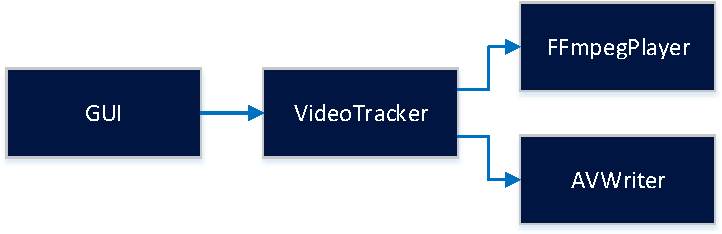
\includegraphics{fig/main_modules}
\caption{Relations among main modules}
\label{fig:main_modules}
\end{figure}
The four modules are described in details in sections below in the order: the FFmpegPlayer in \autoref{ch:ffmpegplayer}, the AVWriter in \autoref{ch:avwriter}, the VideoTracker in \autoref{ch:videotracker} and the Graphical user interface in \autoref{ch:gui}. This is the order in which the modules were designed and implemented as the latter uses the former. Relations among main modules are depicted in \autoref{fig:main_modules}. An arrow points to an object that is controlled by the object the arrow goes from.

%%%%%%%%%%%%%%%%%%%%%%%%%%%%%%%%%%%%%%%%%%%%%%%%%%%%%%%%%%%%%%%%%%%%%%%%%%%%%%%%
\chapter{Media player (FFmpegPlayer)}\label{ch:ffmpegplayer}
\section{Module description}
The media player is a base module the functionality of which is essential for correct application behaviour. It has to support some functions more accurately than simple media players that are used only for media presentation. The ability of the media player to jump to any exactly specified frame as well as reading previous and following frames is crucial. The media player shall support various video formats. That made the design and implementation much more complicated since different video formats mean different information representation and not all methods for frames reading are valid for all video formats.
%\begin{figure}[h]
\begin{figure}[!htbp]
\centering
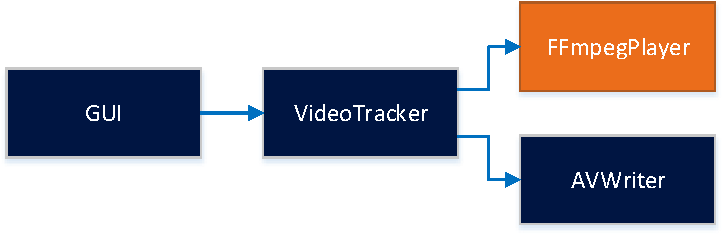
\includegraphics{fig/ffmpegplayer}
\caption{FFmpegPlayer in relations with other main modules}
\label{fig:ffmpegplayer}
\end{figure}

%%%%%%%%%%%%%%%%%%%%%%%%%%%%%%%%%%%%%%%%
\section{Selecting a multimedia library}
\subsection{OpenCV is not sufficient}
The media player was initially implemented in OpenCV~\cite{opencv_essentials} since the particle tracking algorithm uses this library and less conversions would be needed. However, class VideoCapture, which is used in OpenCV for reading video files, does not allow jumping to any desired frame. VideoCapture works correctly only with key frames (key frames are explained in \autoref{subs:keyframes}). Frames which are not key frames are read poorly. Another reason for replacing OpenCV in the media player is that OpenCV works only with video streams. It means that OpenCV cannot either read any audio track, or can it be used for creating any output media file with an audio track. Since an audio track, if present, needs to be processed and stored in the output as well, another media library must be used. It has to be a library that works on a lower level than OpenCV. The FFmpeg library meets this condition; OpenCV's VideoCapture class uses FFmpeg.

\subsection{FFmpeg}
FFmpeg~\cite{ffmpeg_basics} supports various video and audio formats and enables their encoding as well as decoding. Moreover, a strong advantage is that FFmpeg is a cross-platform library\footnote{Cross-platform means that the library can opearate on multiple computer platforms.}. That is the reason why the OpenCV media player was replaced with a player using FFmpeg library, referred as the \keyName{FFmpegPlayer} from now on. Using FFmpeg provides the possibility to adjust the FFmpegPlayer to the needs of the project. On the other hand, working directly with FFmpeg poses other difficulties. Things that were done automatically when using OpenCV (such as selecting the right stream, opening codecs, using video contexts, etc.), are left up to programmers in FFmpeg as it is a low-level library.

\subsection{FFmpeg in the AVWriter}
FFmpeg shall be used also in the AVWriter because it needs to obtain data from the FFmpegPlayer and all superflous conversions shall be avoided. FFmpeg provides all required functionality for media encoding. Thus, FFmpeg seems appropriate for the AVWriter.

%%%%%%%%%%%%%%%%%%%%%%%%%%%%%%%%%%%%%%%%
\section{Media opening}
\subsection{Streams searching}
When a media is being opened in the program it is firstly searched for a video and for an audio stream. Audio stream is optional as it is not used for tracking. Still, an audio stream should be included when creating an output media file if it was present in the input file. Contrarily to an audio stream being optional, a video stream is required. If the media file did not include any video stream, it would not be correctly loaded. There is always found at the most one video and one audio stream. They are always the first ones present in the media file. If the media file contained more video or audio streams, the others would be skipped.

\subsection{Decoder and video context}
After examining media tracks, a decoder is found with FFmpeg’s function \funcName{avcodec_find_decoder()}. When the decoder is found, a video context is copied and its corresponding codec is opened. The video context needs to be copied as the original one must not be used directly. The created video context will keep information about the current position in the video. This is the way the video track is prepared to be correctly decoded and read. The audio track is not handled as the video track because decoding is not needed for it. This is explained in \autoref{sec:audiopackets}. The last step of media opening is a video analysis that is described in \autoref{sec:videoanalysis}.

%%%%%%%%%%%%%%%%%%%%%%%%%%%%%%%%%%%%%%%%
\section{Compressed videos, different types of frames}\label{sec:videocompression}
\subsection{Key frames and non-key frames}\label{subs:keyframes}
As videos are usually memory demanding, most video formats (e.g. MPEG) use a compression technique~\cite{compression_techniques} that does not store full frame’s data for each frame. It uses frames that are called \newExpr{key frames} (referred also as \newExpr{Intra frames}) and frames that are \newExpr{non-key frames}. While key frames contain full image (all data for the frame being displayed), frames that are not key frames consist only of a difference between the particular frame and the preceding frame. This is the way the actual frame’s data can be computed while the amount of data that must be stored is greatly reduced. The reduction is the higher the less changes occur between adjacent frames. Whenever a substantial change has been made, a new key frame needs to be produced. In such a situation an incrementally represented frame would not be of any benefit. This occurs, for example, when a scene is switched.

\subsection{Types of non-key frames}
Non-key frames constitute of two kinds of frames. The first one, called \newExpr{predicted frames}, represents frames that depend on the previous frame. The second kind is \newExpr{bidirectional frames}. Bidirectional frames depend not only on the previous frame but also on the following frame. That way the amount of information to be stored is reduced even more. Typically, videos have a \newExpr{group of pictures (GOP)}. GOP is a structure that specifies what types of frames and in which order are present in a video. Length of such a structure says what the distance between two key frames is. This value is called \newExpr{GOP size}.

\subsection{Presentation and decoding timestamps}\label{subs:timestamps}
However, with non-key frames (especially bidirectional frames) present, video decoding becomes more complicated. A~timestamp saying when a particular frame should be displayed is not sufficient as some frames need to be decoded at different time than they are displayed. In that case, frames cannot be presented immediately after reading. Instead, they are stored in a buffer so that other frames can use their data when needed. That means the order of presentation and decoding is for frames different when bidirectional frames are used. In order to know when a frame should be presented and when decoded, two timestamps exist for each frame~\cite{mpeg_timestamps}. The first one is called \newExpr{presentation timestamp (PTS)}. It says in what order the frames should be displayed. The second timestamp – \newExpr{decoding timestamp (DTS)} says in which order the frames need to be decoded. These timestamps vary only when bidirectional frames are used.
This does not become evident when a video is being played, however, it introduces difficulties when seeking requested frames. Seeking issue is described in \autoref{sec:seeking}.

\begin{table}[h]
  \begin{center}
    \begin{tabular}{ l c  c  c  c  c  c c }
        \textbf{Type:} & K~& B & P & P & P & K~& B\\
        \textbf{DTS:} & 1 & 2 & 3 & 4 & 5 & 6 & 7\\
        \textbf{PTS:} & 2 & 1 & 3 & 4 & 5 & 7 & 6\\
    \end{tabular}
    \caption{Difference between presentation and decoding timestamps with bidirectional frames}
    \label{tab:timestamps}
  \end{center}
\end{table}


Example in \autoref{tab:timestamps} shows the difference between PTS and DTS when all three mentioned kinds of frames are present. Key frames are marked as \keyName{K}, Predicted frames as \keyName{P} and bidirectional frames as \keyName{B}. The key frame with presentation timestamp 2 needs to be decoded before the bidirectional frame with presentation timestamp 1 because the bidirectional frame needs the following key frame for its own decoding. The same happens with the key frame at PTS 7 and the bidirectional frame at PTS 6. GOP size of the structure is 5 (distance between two key frames).

%%%%%%%%%%%%%%%%%%%%%%%%%%%%%%%%%%%%%%%%
\section{Reading frames}\label{sec:reading}
\subsection{Reading correct packets and decoding}\label{subs:decoding}
\funcName{av_read_frame()} is an FFmpeg function that reads the next packet from an opened media~\cite{ffmpeg_dranger}. This packet contains information to which stream it belongs. Since an index of the video stream was discovered when opening the media, packets belonging to streams with different indices can be skipped. Correct packets (packets from the video stream) are then decoded with \funcName{avcodec_decode_video2()}. This is a function provided by FFmpeg for decoding video frames. The frame returned by the function does not necessarily correspond to the packet that was currently passed as an argument to the function. Packets are read by \funcName{av_read_frame()} in the order in which they are stored in the video track. The returning order might be different. \funcName{avcodec_decode_video2()} internally decodes frames according their timestamps for decoding so that frames have all information from other already decoded frames needed for their decoding available. Returned frames are ordered by their presentation timestamps. That means the returned frame is the one that should be currently presented. Reasons for these two kinds of timestamps are described in \autoref{subs:timestamps}

\subsection{Buffers}
Given the fact that some frames that are supposed to be presented later than others are decoded earlier, \funcName{avcoded_decode_video2()} might not return any frame when first packets are passed to this function. Only when it has all information that were needed for decoding the frame that should be presented, it returns this first frame. Thus, it takes several video packets to be read before the first video frame is displayed. After this initial procedure, \funcName{avcoded_decode_video2()} returns a frame with every passed new packet.
Moreover, when all packets were read with \funcName{av_read_frame()}, it does not mean that all frames were displayed. It is important to call \funcName{avcoded_decode_video2()} even without passing new packets because it still contains decoded frames. The amount of the remained frames equals the number of packets that had to be passed to \funcName{avcoded_decode_video2()} before it started returning decoded frames. This ensures that the number of displayed frames corresponds with the number of read frames.

%%%%%%%%%%%%%%%%%%%%%%%%%%%%%%%%%%%%%%%%
\section{Seeking frames}\label{sec:seeking}
\subsection{FFmpeg functions for seeking}
Frame seeking is in FFmpeg provided by a function \funcName{av_seek_frame()}. This function seeks a frame in a video based on the frame’s timestamp. If the timestamp is not known, an approximate timestamp can be computed by \funcName{av_rescale_q()}. It takes a time value and converts it to the video stream’s time base. After a frame is sought, it can be read by a function \funcName{av_read_frame()}. This function reads the next frame. Without calling \funcName{av_seek_frame()} it always reads the frame following to the current one. When \funcName{av_seek_frame()} is used, \funcName{av_read_frame()} reads the sought frame. However, it is necessary to flush buffers with \funcName{avcodec_flush_buffers()} before reading in this situation because they contain frames stored before seeking was executed. Buffers are used because of video compression. This is explained in \autoref{sec:videocompression}.

\subsection{Seeking key frames}
Frames should not be difficult to seek if we know either their timestamp or their time position and do not forget to flush buffers. However, a problem occurs if the frame we want to seek is not a key frame. Seeking situations are explained on graphical examples. Symbols used in these examples are shown shown in \autoref{fig:seek_marks} and their meanings are: 1) key frame, 2) non-key frame, 3) returned key frame, 4) returned non-key frame, 5) sought key frame 6) sought non-key frame 7) Returned incomplete frame, 8) Reading a next frame with \funcName{av_read_frame()}.
%\begin{figure}[h]
\begin{figure}[!htbp]
\centering
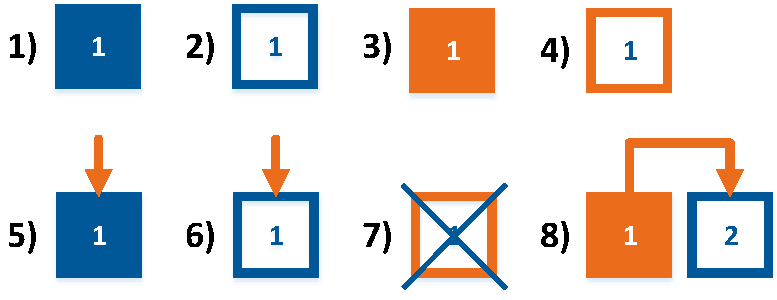
\includegraphics[scale=0.6]{fig/seeking_marks}
\caption{Marks that are used for describing seeking situations}
\label{fig:seek_marks}
\end{figure}

%\begin{figure}[h]
\begin{figure}[!htbp]
\centering
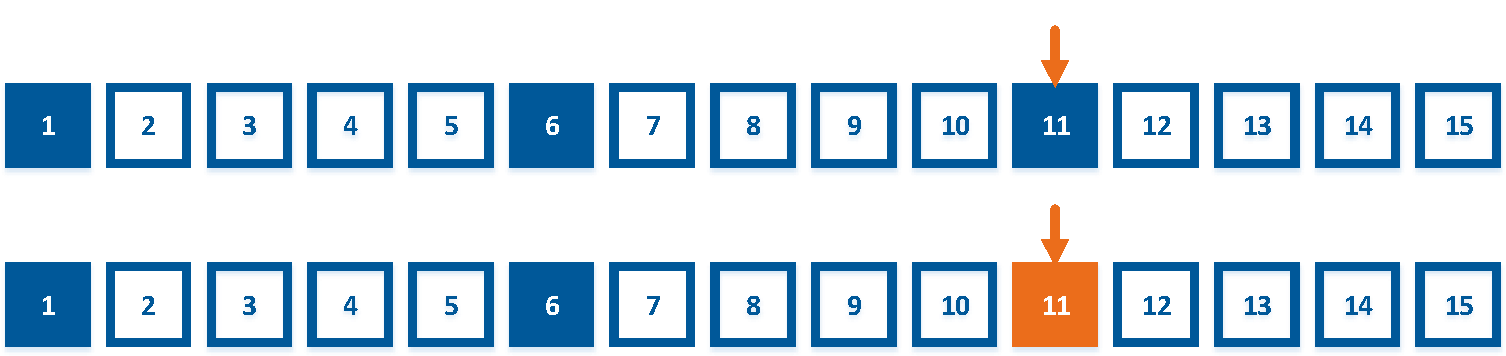
\includegraphics[width=\textwidth]{fig/seeking_key}
\caption{Seeking a key frame}
\label{fig:seek_key}
\end{figure}
\funcName{av_seek_frame()} can be set to seek either all frames or only frames that are key frames. The latter is shown in \autoref{fig:seek_key} and \autoref{fig:seek_nonkey}.
If the sought timestamp belongs to a key frame like in \autoref{fig:seek_key}, where the sought timestamp is 11, the returned frame has a timestamp 11 as well. However, if the sought timestamp does not belong to a key frame, the closest key frame is returned.
%\begin{figure}[h]
\begin{figure}[!htbp]
\centering
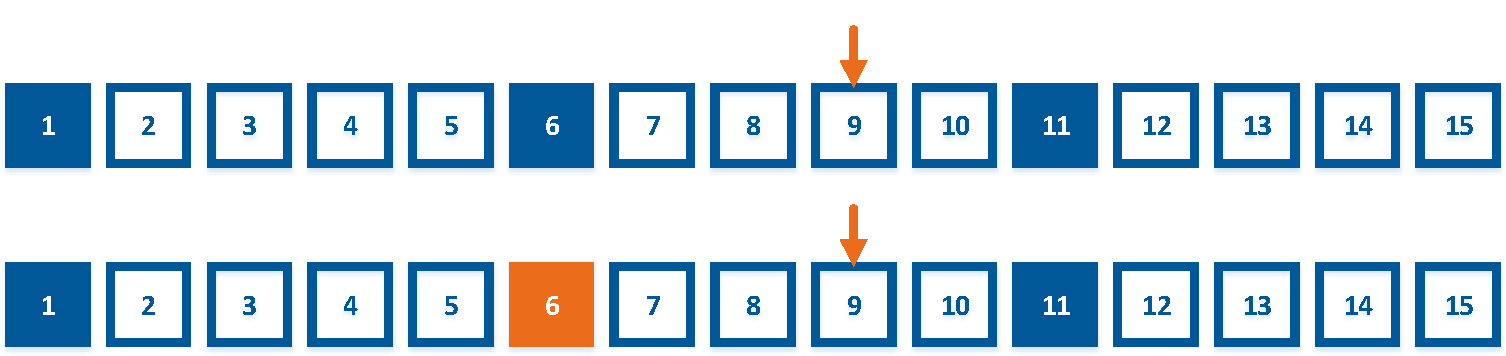
\includegraphics[width=\textwidth]{fig/seeking_non_key}
\caption{Seeking a non key frame with flags set for seeking only key frames}
\label{fig:seek_nonkey}
\end{figure}
The \autoref{fig:seek_nonkey} shows seeking a non-key frame with a timestamp 9 while a key frame with its timestamp 6 is returned (when seeking backward). Still, this is usually sufficient because \funcName{av_seek_frame()} is mostly used for jumping to a certain time position where a media player continues playing a video. In such a situation exact position is not required as a position that differs maximally a few seconds from the asked time position is acceptable and is barely visible to users. The maximal difference depends on the GOP size of a video. For example, if a video has a key frame each 12th frame (GOP size is 12) and 24 frames should be displayed per second (fps value is 24), the difference between requested and actual frame is always lower than 0.5 second (12/24 s). Since seeking frames at exact positions is essential for this project, this behaviour is not acceptable; seeking frames that are not key frames must work as well.
Even when \funcName{av_seek_frame()} is set to seek any frame (not just key frames), obtained frame is not complete unless it is a key frame. Non-key frames need to be computed from the other frames. Seeking in FFmpeg is simple and does not cope with this situation. FFmpeg returns complete images when reading with \funcName{av_read_frame()} providing it started reading from a key frame. Thus, if \funcName{av_seek_frame()} is used only for seeking key frames, frames are always complete.

\subsection{Non-key frames cannot be sought directly}
Even when \funcName{av_seek_frame()} is set to seek any frame (not just key frames), obtained frame is not complete unless it is a key frame. Non-key frames need to be computed from the other frames. Seeking in FFmpeg is simple and does not cope with this situation. FFmpeg returns complete images when reading with \funcName{av_read_frame()} providing it started reading from a key frame. Thus, if \funcName{av_seek_frame()} is used only for seeking key frames, frames are always complete. If a non-key frame was seeked directly like the frame with a timestamp 9 in \autoref{fig:seek_nonkey_incomplete}, it would be returned but such a frame is incomplete and thus cannot be shown.
%\begin{figure}[h]
\begin{figure}[!htbp]
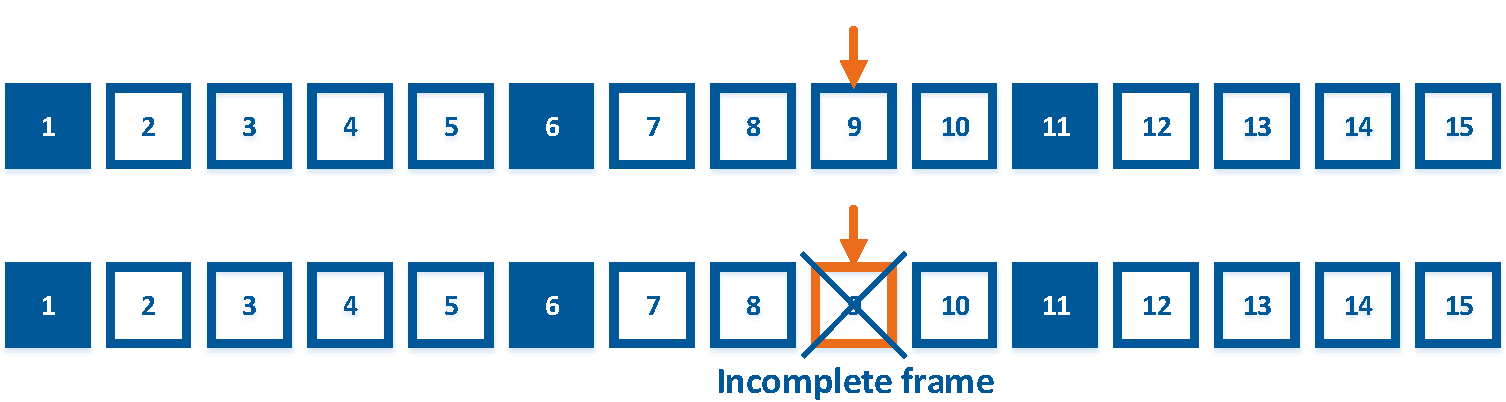
\includegraphics[width=\textwidth]{fig/seeking_non_key_incomplete}
\caption{Seeking a non key frame with flags set for seeking all frames results in an incomplete frame}
\label{fig:seek_nonkey_incomplete}
\end{figure}

\subsection{Seeking all frames (key frames and non-key frames)}
For a sought non-key frame to be complete, the previous key frame needs to be sought and by reading next frames with \funcName{av_read_frame()} and decoding them with \funcName{avcodec_decode_video2()} the requested frame is reached with its data being valid. It is now possible to get any frame when having its previous key frame. \funcName{av_seek_frame()} can be set to seek either forward or backward with relation to a given timestamp. Setting flags to seeking backward and seeking only key frames results in finding a key frame that is either at the requested position or time position before. This is the way the previous key frame is found when the requested frame is not a key frame. And the requested frame is reached as described above. 
%\begin{figure}[h]
\begin{figure}[!htbp]
\centering
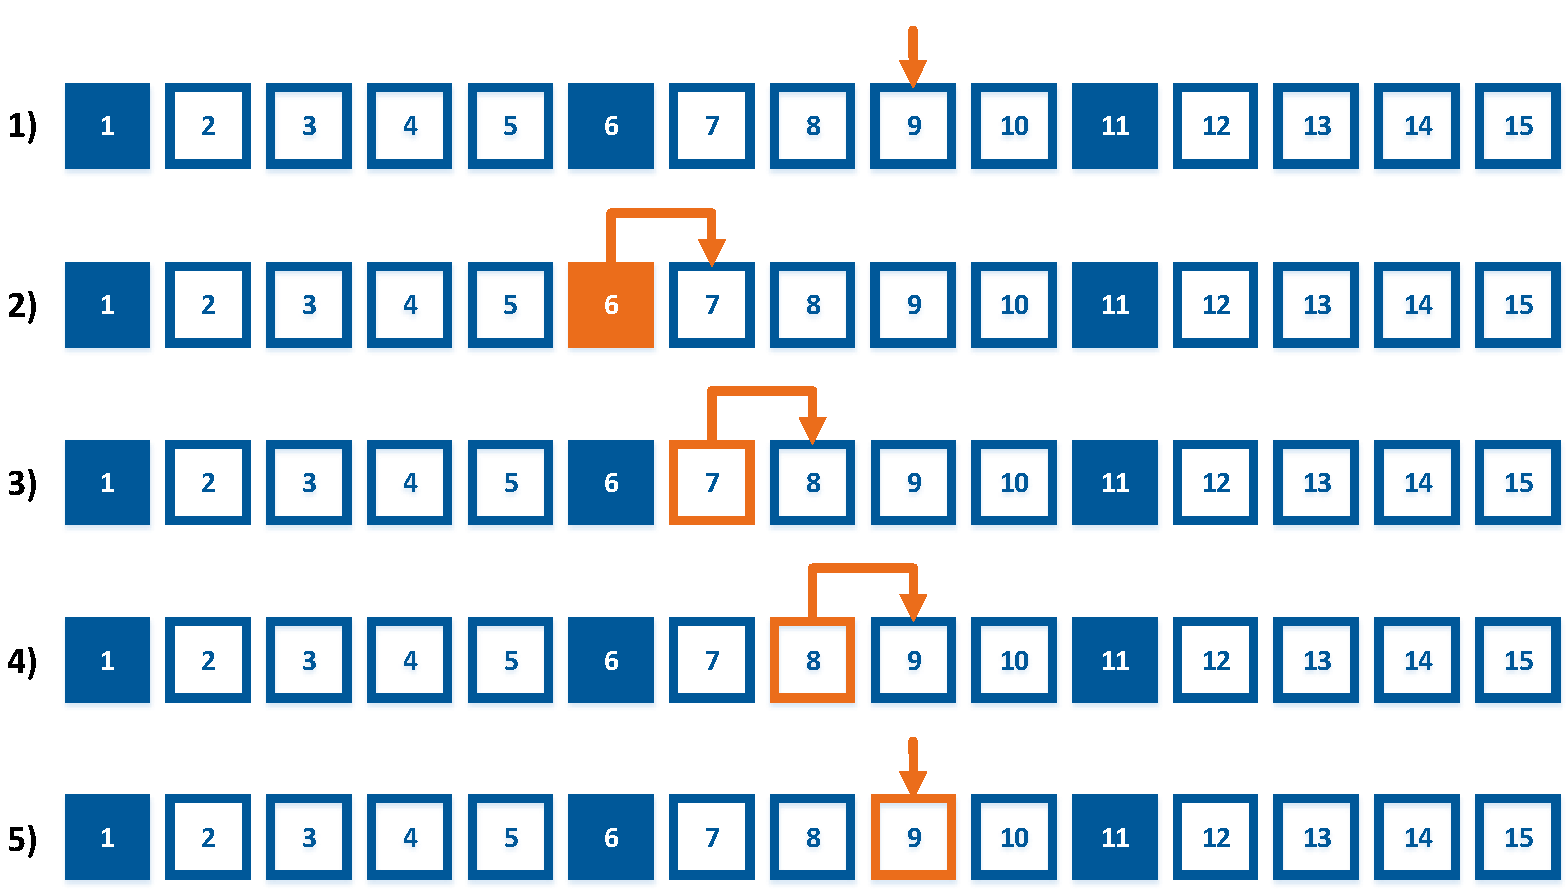
\includegraphics[width=\textwidth]{fig/seeking_algorithm}
\caption{An algorithm used for seeking all frames}
\label{fig:seek_algorithm}
\end{figure}
Reading non-key frames is described in \autoref{fig:seek_algorithm}. In the first step a frame with a timestamp 9 is sought but flags are set to be seeking only key frames and seeking backward. A~key frame with a timestamp 6 is returned. After that \funcName{av_read_frame()} is used as many times till the frame with its timestamp 9 is reached.

\subsection{Inaccurate seeking needs to be checked}
Yet, seeking in FFmpeg is inaccurate for some videos. Even when seeking backward, the sought frame has sometimes a timestamp higher than requested. It is necessary to check for this situation and try seeking lower when this occurs. This means that the video has to be analysed upon opening to have information about timestamps of all frames. The video analysis is described in \autoref{sec:videoanalysis}. Procedure for handling seeking inaccuracy is shown in \autoref{fig:seek_inaccurate}. Frame with its timestamp 9 was sought. Despite seeking backward a key frame with its timestamp 11 is returned. That is the reason why a frame with a lower timestamp (9) was sought. Again, the returned frame's timestamp is higher than expected and seeking lower must be made. This is done until the returned frame's timestamp is lower; in this example seeking a frame with its timestamp 7 returned a key frame with its timestamp 6. This is correct and an algorithm in the \autoref{fig:seek_algorithm} can be executed.
%\begin{figure}[h]
\begin{figure}[!htbp]
\centering
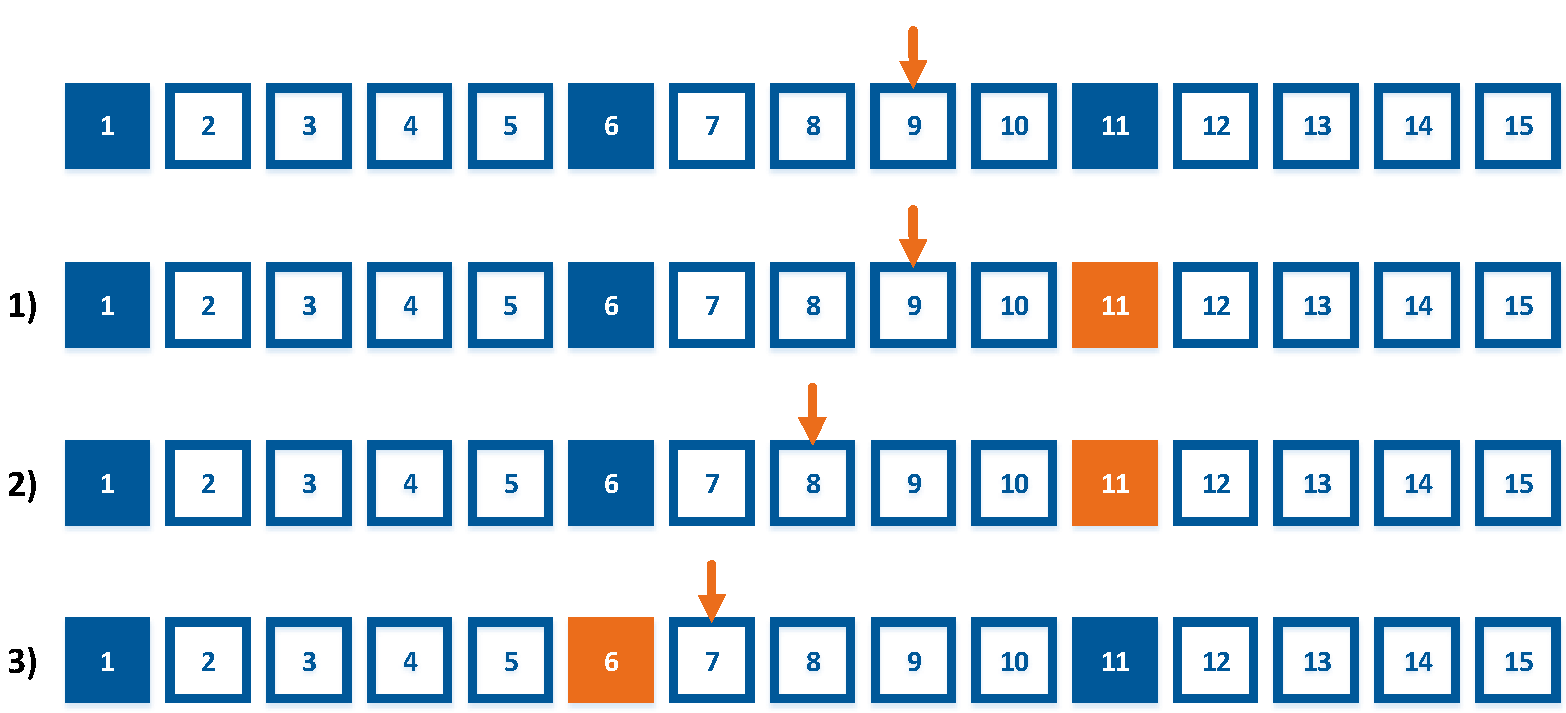
\includegraphics[width=\textwidth]{fig/seeking_inaccurate}
\caption{Correction of seeking inaccuracies}
\label{fig:seek_inaccurate}
\end{figure}

\subsection{Final seeking algorithm}
When knowing timestamps of all frames, reading a certain frame goes as follows:
\begin{enumerate}
\item Timestamp of the frame is determined if its index is provided, otherwise the provided timestamp is used.
\item Frame is sought by its timestamp with the function \funcName{av_seek_frame()} with flags set for seeking only key frames and seeking backward.
\item The returned frame is read and its timestamp is checked. If the timestamp is higher than the requested timestamp, seeking is not successful and must be made again with a lower timestamp. That means seeking with the previous timestamp to the requested timestamp. This needs to be done as many times until the condition (returned timestamp is lower than or equal to the originally requested timestamp) is true.
\item If the returned frame’s timestamp is equal to the requested one, the frame is successfully read and can be returned.
\item Otherwise (if the returned frame’s timestamp is lower than the requested one), \funcName{av_read_frame()} is called as many times until a frame with the requested timestamp is reached. This frame is then returned.
\end{enumerate}
Step 3 is needed only because of \funcName{av_seek_frame()} not behaving correctly. It is not supposed to return a frame with timestamp higher than requested when seeking backward.

Given the fact the seeking issue is now solved, it is possible to jump to any frame by its timestamp, index as well as by its time position (a time position is rescaled to a timestamp by \funcName{av_rescale_q()}). Seeking is used also when jumping to the beginning of the video; it simply seeks the first frame in the video stream. FFmpeg does not provide a function for a step back either. That is the reason why stepping back is implemented as seeking the previous frame. Yet, stepping forward does not use seeking. When frames are read consecutively, standard FFmpeg function \funcName{av_read_frame()} is used without any seeking. Thus, stepping forward is the most efficient way of reading a frame.


%%%%%%%%%%%%%%%%%%%%%%%%%%%%%%%%%%%%%%%%
\section{Obtaining number of frames}\label{sec:numframes}
\subsection{Incorrect information}
Despite the fact that videos provide an information about their number of frames, this information is not always accurate. For example, some video files might be incomplete. Such files would claim to have a certain number of frames when the actual number is lower. FFmpeg simply returns the number of frames a video file provides without verifying it.

\subsection{Considered solution 1: Continuous updating}
The solution would be to use the claimed number of frames and update such an information when inaccuracy was found while working with the video. For example, if the claimed number of frames was 250, the video was being played and stopped at the frame number 230 with the information that there were no more frames to read, the FFmpegPlayer would remember this information as the actual number of frames. This should be sufficient for the VideoTracker, however, if displaying the number of frames to users, they might be getting inaccurate information before the FFmpegPlayer reaches the actual end of the video.

\subsection{Considered solution 2: Seeking last frame}
Another considered option is to seek the last frame and read its index. However, frames are distinguished by their timestamps, not indices. In some video formats, timestamps are considered to be indices whereas in some formats not. Therefore, it is not possible to use timestamps for obtaining the number of frames in a video. Moreover, since seeking in FFmpeg is done by frames’ timestamps, it is not possible to read the last frame when not knowing its timestamp or its time position (a time position might be used for counting timestamp).

\subsection{Selected solution: Analysing video upon opening}
Finally, an accurate option is to go through all frames when opening a video and count their number. Even though opening would take longer in such a case, it would be outweighed by knowing the actual number of frames. Given the fact that the previous options were not sufficient, this is the selected one. A~video analysis is required for this solution. The analysis is described later in \autoref{sec:videoanalysis}.


%%%%%%%%%%%%%%%%%%%%%%%%%%%%%%%%%%%%%%%%
\section{Video analysis}\label{sec:videoanalysis}
A~video analysis is performed not only for obtaining a correct number of frames but also for preparing a video to be seekable. The analysis means reading next frames from the first frame of the video till the end and storing timestamps of all frames. Knowing frames’ indices would also be beneficial if stored with timestamps. It would enable seeking frames by their index. Since no decoding is done during the analysis, as it would make the video opening much slower, frames are not in the presentation order but in the order in which they should be decoded. This is explained in \autoref{subs:timestamps}. This means there might be frames with lower presentation timestamps that were not yet read while a frame with higher timestamp has already been analysed. That is the reason why their indices cannot be determined immediately. Therefore, timestamps (presentation timestamps) are in the program stored in a C++ std::set that sorts the values. After reading all frames a C++ std::vector with timestamps is also created. This is the way timestamps can be determined by frames’ indices and vice versa.

%%%%%%%%%%%%%%%%%%%%%%%%%%%%%%%%%%%%%%%%
\section{Audio packets}\label{sec:audiopackets}
The VideoTracker does not need audio packets for tracking objects in a video. Because of that only video frames are processed. The audio packets are thus skipped by the FFmpegPlayer with one exception; if an output video is being created, the audio track should be present in the output as well. Therefore, the function for reading frames in the FFmpegPlayer can be set to reading either only a video track or the video track as well as an audio track. Read video packets are always decoded since the VideoTracker works with frames, not packets. For audio packets this does not apply. There is no need for decoding them as they are used only for creating the output. Output creating is in detail described in \autoref{ch:avwriter}.

%%%%%%%%%%%%%%%%%%%%%%%%%%%%%%%%%%%%%%%%%%%%%%%%%%%%%%%%%%%%%%%%%%%%%%%%%%%%%%%%
\chapter{Media writer (AVWriter)}\label{ch:avwriter}
\section{Module description}
The AVWriter is a module containing logics for creating an output media file. It is controlled by the VideoTracker that receives frames and packets from the FFmpegPlayer, processed them and gives them to the AVWriter to write them to the output media file. The AVWriter uses the FFmpeg library just like the FFmpegPlayer.
%\begin{figure}[h]
\begin{figure}[!htbp]
\centering
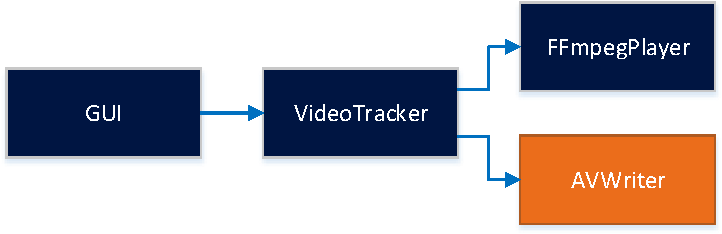
\includegraphics{fig/avwriter}
\caption{AVWriter in relations with other main modules}
\label{fig:avwriter}
\end{figure}

%%%%%%%%%%%%%%%%%%%%%%%%%%%%%%%%%%%%%%%%
\section{Output file format and contexts}
The format of an output video file is chosen by the input video format. If the format is not supported by FFmpeg for creating a media file, MPEG is used instead. Afterwards, an encoder has to be found so that output streams (a video stream and an audio stream) could be created. When the streams are created, their contexts have to be prepared. Information from input contexts are used for settings the output contexts. When this is done, streams are ready for writing packets. 

%%%%%%%%%%%%%%%%%%%%%%%%%%%%%%%%%%%%%%%%
\section{Writing video frames}
The VideoTracker receives frames from the FFmpegPlayer that are already decoded so they can be processed. When these frames are being written in the output media file, they need to be encoded back. This is done by a function \funcName{avcodec_encode_video2()} that is provided by FFmpeg. It takes a raw frame and encodes it into a packet. This function is a reverse function to the function \funcName{avcodec_decode_video2()} that was described in \autoref{subs:decoding}. The buffers work also very similarly. When raw frames are being passed to \funcName{avcodec_encode_video2()}, it does not return any encoded packet at the beginning. The buffer needs to be filled first. When the buffer is filled, it returns an encoded packet for each passed raw frame. It is very important to empty the buffer after all the frames were passed because the buffer still contains encoded packets.

%%%%%%%%%%%%%%%%%%%%%%%%%%%%%%%%%%%%%%%%
\section{Writing audio packets}
Audio packets were not decoded in the FFmpegPlayer because no processing was required. Therefore, the VideoTracker passes them to the AVWriter exactly the same as they were read by the FFmpegPlayer. The AVWriter does not do any encoding because the packets are already encoded. Simple adding to the audio stream is performed. This makes the output creation much faster because decoding and encoding are the most demaning processes when creating an output.


%%%%%%%%%%%%%%%%%%%%%%%%%%%%%%%%%%%%%%%%%%%%%%%%%%%%%%%%%%%%%%%%%%%%%%%%%%%%%%%%
\chapter{Video tracker (VideoTracker)}\label{ch:videotracker}
\section{Module description}
The core of the application is a module called a \keyName{VideoTracker}. This module shall control opening videos and reading frames by the FFmpegPlayer (\autoref{ch:ffmpegplayer}) as well as creating an output video file with the AVWriter (\autoref{ch:avwriter}). The VideoTracker includes all the logic for tracking and anonymizing objects. It is controlled directly by the MainWindow module (\autoref{ch:gui}) that is not allowed to communicate with the FFmpegPlayer and the AVWriter.
%\begin{figure}[h]
\begin{figure}[!htbp]
\centering
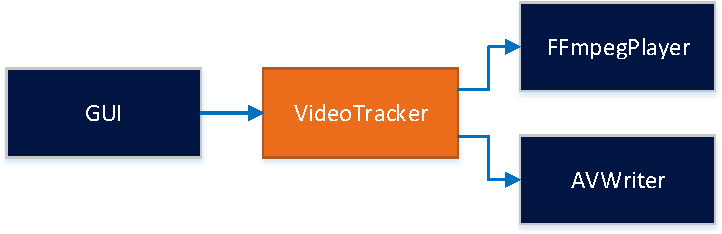
\includegraphics{fig/videotracker}
\caption{VideoTracker in relations with other main modules}
\label{fig:videotracker}
\end{figure}

%%%%%%%%%%%%%%%%%%%%%%%%%%%%%%%%%%%%%%%%
\section{Frames conversions (VideoFrame)}\label{sec:videoframe}
\subsection{Different frame formats}
FFmpeg works with frames in its AVFrame format. However, this format cannot be used for tracking as the VideoTracker works with OpenCV library. OpenCV supports its own cv::Mat and IplImage formats. IplImage should be used only in cases when cv::Mat is not supported since cv::Mat is a newer and preferred format. Conversions between cv::Mat and IplImage are handled automatically by OpenCV. Conversions from AVFrame to cv::Mat and back are more complicated. Converting from AVFrame to cv::Mat is needed when a frame that is read by the FFmpegPlayer is used by the VideoTracker. Conversion back to AVFrame is used only when an output video file is being created.

\subsection{New module}
Since the FFmpegPlayer is implemented in FFmpeg and the VideoTracker in OpenCV, the conversions should be made outside both this modules. That is the reason why another class should be created that could be used by both the FFmpegPlayer as well as the VideoTracker. This class would include a frame and would be able to provide it in a requested format; either AVFrame or cv::Mat. This class is in the project called a \keyName{VideoFrame}.
%\begin{figure}[h]
\begin{figure}[!htbp]
\centering
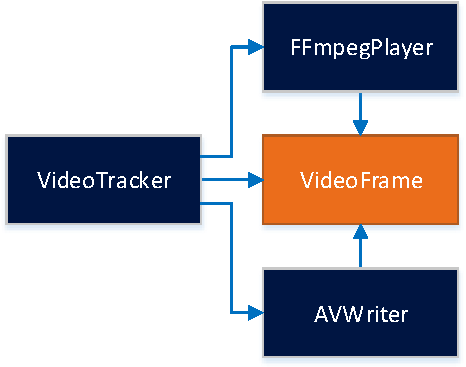
\includegraphics{fig/videoframe}
\caption{VideoFrame in relations with main modules}
\label{fig:videoframe}
\end{figure}

\subsection{Converting AVFrame to cv::Mat}
A~VideoFrame is always set by a frame in AVFrame format. The VideoFrame converts this frame to cv::Mat and stores it. The conversion is done by calling \funcName{sws_scale()} that converts the AVFrame from one format to another. The source format is the one of the original frame (e.g. YUV420P). The destination format is the format used by OpenCV; BGR24. Since \funcName{sws_scale()} cannot convert directly from AVFrame to cv::Mat, an auxiliary destination AVFrame is created. Its data pointer is set to be the pointer to the cv::Mat’s data. \funcName{sws_scale()} this way works with the cv::Mat while seeing it as an AVFrame. Before the actual conversion a conversion context needs to be prepared with \funcName{sws_getContext()}. Beside setting source and output formats, picture’s size is in the context defined to be preserved. When the conversion is finished, the VideoFrame contains a cv::Mat picture that can be used for tracking.

\subsection{Converting cv::Mat to AVFrame}
Conversion back to AVFrame happens only when a VideoFrame is asked to return this format. This occurs when the frame is being encoded to be added to an output video stream in the AVWriter. Conversion from cv::Mat to AVFrame is similar to the inverse one. An auxiliary AVFrame source is created and set to point to the cv::Mat source. Correct conversion context is set and \funcName{sws_scale()} is called.

\subsection{Other stored data}
Since cv::Mat does not include any information apart from a picture itself, other data need to be stored directly in a VideoFrame and provided on demand. Data that are needed together with a picture are frame’s timestamp, frame’s number (index) and its time position. The FFmpegPlayer gives the VideoFrame all this information. The frame’s number is discovered from the data obtained when analysing the video at its opening and the time position is computed from the frame’s timestamp based on a time base of a video.

%%%%%%%%%%%%%%%%%%%%%%%%%%%%%%%%%%%%%%%%
\section{Displaying frames}
\subsection{Processing frames}
When a frame shall be displayed, the VideoTracker asks the FFmpegPlayer for this frame. Once received, the VideoTracker handles frame's editing with respect to tracked objects. All FFmpeg functions for reading frames are wrapped in VideoTracker's functions that take care of drawing tracked objects when present.

\subsection{Converting cv::Mat to QImage}\label{subs:mat2qimage}
A~frame in cv::Mat format has to be converted to QImage so that it can be displayed in the graphical user interface that uses QT framework. First step of the conversion is to transform a BGR\footnote{Blue, Green, Red} format, that is used in OpenCV, to RGB\footnote{Red, Green, Blue} format that is used in QT. After this transformation, a new QImage structure is set to be prepared for the frame data from the cv::Mat. The last step is making a deep copy of the cv::Mat data and filling the QImage.

%%%%%%%%%%%%%%%%%%%%%%%%%%%%%%%%%%%%%%%%
\section{Tracking algorithm}\label{sec:trackingalgorithm}
\subsection{Particle tracking algorithms}
Particle tracking algorithms are algorithms that use particles for objects tracking~\cite{particle_tracking}. One method that uses particles is called a Kalman filter. A problem with this method is that only one candidate for a tracked object can be selected at a time. A reason for this is that the distribution is Gaussian. A method that solves this issue is called a Particle filter. Unlike the Kalman filter, the Particle filter uses the Monte Carlo method that enables modelling cases that are not Gaussian. This method is used in this application.

\subsection{TrackingAlgorithm}
The application uses a provided particle tracking algorithm for tracking objects in a video~\cite{algorithm_thesis}. The algorithm was divided into an initialization part and a part for tracking the next frame for purposes of this application. The initialization was adjusted to be done according an initial frame's data and the initial position of the tracked object. The second part, tracking the next frame, takes only frame's data and returns the object's position. The algorithm is located in a module called a \keyName{TrackingAlgorithm}. The module expects to be provided with following frames when no frame is skipped. The module's interface does not depend on this particular algorithm so the algorithm might be easily replaced by a different one.

%%%%%%%%%%%%%%%%%%%%%%%%%%%%%%%%%%%%%%%%
\section{Tracked objects (TrackedObject)}
\subsection{Module description}
Since multiple objects tracking shall be enabled, it is necessary to create a new module, that holds information about and logic for maintaining each object. This module is called \keyName{TrackedObject}. It is controlled by the VideoTracker and for passing frames uses the VideoFrame. Each object consists of sections called a \keyName{TrajectorySection}. They are described in \autoref{subs:sections}. These sections use the TrackingAlgorithm, described in \autoref{sec:trackingalgorithm}.
%\begin{figure}[h]
\begin{figure}[!htbp]
\centering
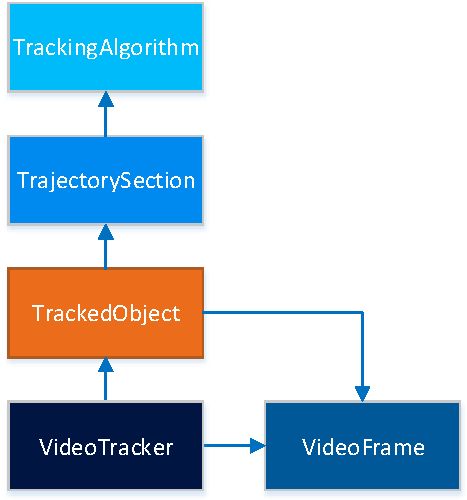
\includegraphics{fig/trackedobject}
\caption{TrackedObject in relations with other modules}
\label{fig:videoframe}
\end{figure}

\subsection{Storing objects' trajectories}
When an object is added for tracking, the only necessary information is the frame where the tracking shall begin and the object's position in this frame. The tracking algorithm is able to compute the object's trajectory from this initial information. To reduce the computation, the computed trajectory is continuously being stored so that computing of the same frames did not have to be done again. When a frame with already computed objets' positions is read, the positions are found in saved trajectories. If a trajectory correction was made, only position at the particular frame would be changed. Since it is desired that the correction applies till the end of the object's lifetime, the trajectory has to be cut into sections.

\subsection{Sections}\label{subs:sections}
Each section represents a part of an object's trajectory with a fixed initial position. This means that the section is defined by a frame's timestamp where the section begins and by the object's position in this frame. Each section has its own instance of the TrackingAlgorithm since the TrackingAlgorithm has to be initialized by the first frame's data and coordinates of the tracked object. The end of a section is not defined but it is discovered by examining initial frame's timestamp of the next section. A~section is always valid until the beginning of the following section. If no following section exists, the section is valid till the end of the object's lifetime. When a new object is being tracked and no trajectory corrections are made, only one section exists for this object. Each trajectory correction results in a new section. Only one section is active in a TrackedObject at a time. The TrackedObject takes care of switching the activity when another section is reached. However, all previous sections need to be computed before switching to the next section. Thus, the computed trajectory is always continuous.

\subsection{Trajectory correction}
Correcting a trajectory means adding a new section. When a new section is added, the trajectory that has already been computed for the object has to be checked. If the timestamp of the last computed frame is lower than the timestamp of the new section's initial frame, the TrackedObject's state can be preserved. Otherwise, a part of the computed trajectory is not valid because it is interfered by the new section. This part of the trajectory has to be erased and computed again. The currently active section also has to be changed.

\subsection{Removing and modifying sections}
When a section is being removed, the already computed trajectory and a TrackedObject's state has to be checked and updated because the previous section has to be expanded to cover the removed section's interval. If the removed section is the first one, no previous section exists so no section is changed. The removal causes that the following section becomes the first section in the TrackedObject. If a section is modified, the procedure is similar to removing a section followed by adding a new one.

%%%%%%%%%%%%%%%%%%%%%%%%%%%%%%%%%%%%%%%%
\section{Anonymizing / highlighting objects}
\subsection{Drawing an object}
The purpose of this application is to anonymize or highlight tracked objects. Each object shall have its own appearance. This is the reason why objects are drawn in a frame in the TrackedObject module. The TrackedObject includes settings of the drawn object appearance. The appearance shall support various options to suit different application purposes. That is the reason why various shapes and colours can be set.

\subsection{Object shapes and colors}
Two object shapes are supported in the application; a rectangle and an ellipse. Both these shapes can be set to be either filled with a color, marked with a border or to use both these options. Colors of filling and of a border can be set separately. Objects are drawn with the OpenCV library.

\subsection{Anonymizing by defocusing}
Usually, it is not necessary to fill the object with a color for hiding it. It seems unnatural in a video. Instead of filling the object with a color, defocusing it would do the effect of anonymization and would be less disruptive. The defocusing is also implemented in OpenCV. The object's area is divided into blocks. Each block is filled with its mean color. The size of blocks can be adjusted to make the object more or less visible. The process of defocusing must use two pictures. The first one is the original frame and it is used for computing mean color values of blocks. The second one is an altered frame containing drawn objects. The second picture cannot be used for computing mean values because it could be already altered by other objects.

%%%%%%%%%%%%%%%%%%%%%%%%%%%%%%%%%%%%%%%%%%%%%%%%%%%%%%%%%%%%%%%%%%%%%%%%%%%%%%%%
\chapter{Graphical user interface (MainWindow)}\label{ch:gui}
\section{Module description}
The graphical user interface shall be implemented separately from the rest of the application. This is the way the application could be easily rewritten if a different framework for GUIs should be used. It also makes maintaining the GUI easier since this module contains all the graphics and information that are shown to users. It shall include the least application logic possible so the programme is not much dependent on the GUI. That is the reason why the GUI module communicates only with the VideoTracker, the core of the application.
%\begin{figure}[h]
\begin{figure}[!htbp]
\centering
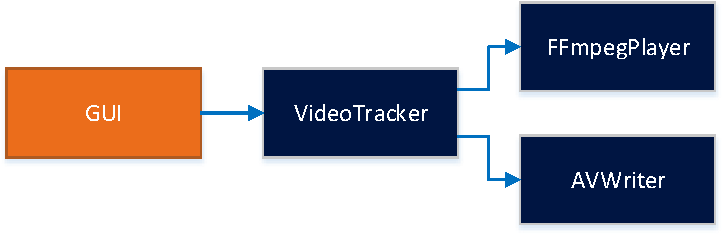
\includegraphics{fig/gui}
\caption{GUI in relations with other main modules}
\label{fig:gui}
\end{figure}

%%%%%%%%%%%%%%%%%%%%%%%%%%%%%%%%%%%%%%%%
\section{QT framework}
\subsection{Reasons for choosing QT}
The GUI is implemented with support of the QT library~\cite{qt_programming}. QT is a cross-platform library for graphical user interfaces that is widely used with C++ applications. The application shall run on various range of platforms. Thus, QT is suitable for the GUI module of this application. QT provides very good support that would be of a good use when developing this application. As mentioned earlier, QT shall be used only in the GUI module so that the rest of the application shall not dependent on it.

\subsection{Signals and slots}
QT uses its signals and slots for connecting events with actions. This handles user's inputs even when the application is busy without any need for a separate thread. All buttons and widgets have signals that are sent whenever these items change their state (e.g. a button is clicked). These signals are then connected with slots (procedures) that are carried out whenever a corresponding signal is sent. This technique is in the application used also when playing a video for showing next frames. This is handled by a timer and it is described in \autoref{subs:timer}.

%%%%%%%%%%%%%%%%%%%%%%%%%%%%%%%%%%%%%%%%
\section{GUI structure}
\subsection{Main parts}
As already mentioned, the FFmpegPlayer (\autoref{ch:ffmpegplayer}) is a fundamental part of the programme and the other modules were built upon it. Even an appearance of the graphical user interface (GUI) is based on a video player. The reason is as follows; when no object is being tracked, the program should behave as a common video player. Most video players look alike and this one should not differentiate much.
\begin{figure}[!htbp]
\centering
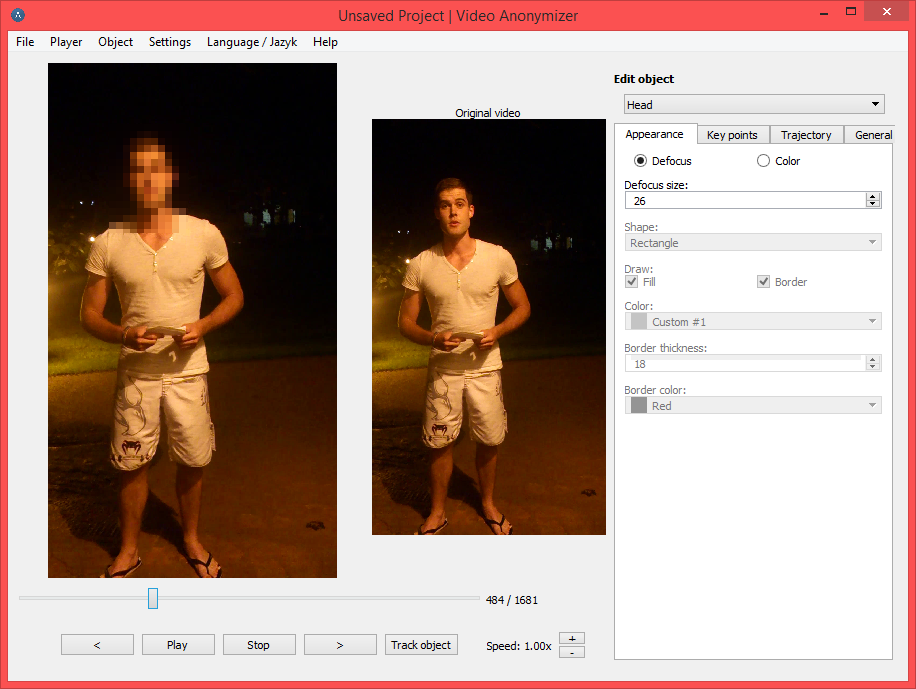
\includegraphics[width=\textwidth]{png/all_defocus}
\caption{An application window where one object is being tracked and its appearance is set to be defocused}
\label{fig:all_defocus}
\end{figure}
If the program is similar to video players that users usually work with, they do not need to focus on the player’s behaviour and they are able to control it without major difficulties. This makes the transition from a video player to this video tracker smoother. That is the reason why the GUI consists of three main parts; the player, an application menu and a tracked objects’ panel. All these parts are visible no matter in what state the GUI currently is. All of them have their own place and do not cover the others. Still, not all features for setting tracked objects’ are visible at the same time as they are placed in tabs that can be switched.

\subsection{Application resolution}
The application shall support various resolutions. Even application resizing needs to be handled. QT provides widgets called \newExpr{Spacers}. These spacers can be described as springs that are stretched when there is an empty space. They are used in the application for maintaining application's appearance regardless different resolutions while using the most of the available space.

\subsection{Video player}
The video player consists of a video frame, controls, position slider and a speed indicator. The video frame displays a current video frame according to a state of the FFmpegPlayer. If a tracked object has been added and affects this frame, the original frame is altered to be displayed with the object. However, this is handled by the VideoTracker so the GUI player displays an original frame the same way as an altered one. The only situation when a video frame needs to be altered by the GUI player is when a selection of a tracked object is being made. This is explained in \autoref{sec:selection}. State of the FFmpegPlayer and thus the displayed video picture is controlled by controls and a position slider that are placed next to the video frame to create a compact player.

%%%%%%%%%%%%%%%%%%%%%%%%%%%%%%%%%%%%%%%%
\section{Position slider}
\subsection{Purposes}
The position slider has two purposes. The first one is an indicator what the current frame’s position in the video track is. The second purpose is for users to select a position in the video track to jump to. Initially, when the FFmpegPlayer was implemented without returning the exact number of frames, positions of the slider represented time values. This was not very accurate because the number of values of the slider did not correspond to the number of frames. An information about a length of a video is available, however, this value would need to be used with an information about fps\footnote{Frames per second}. Computed values would be approximate and together with the fact that some video formats support video frames of various duration, this method would not be convenient for the purpose of this application as it would not allow jumping to exact positions in videos where each frame matters. Besides, the information about a length of a video provided by videos might be as inaccurate as the information about the number of frames as explained in \autoref{sec:numframes}.

\subsection{Frames' indices}
Instead of time positions, timestamps could be used. The FFmpegPlayer has an information about all frames’ timestamps. If timestamps are used as values of the slider it is possible to determine each frame. Still, timestamps are not the best choice. Slider values should be continuous; each two neighbouring values shall have the same distance, i.e. one. Frames’ indices comply with this condition. The first frame has an index with value 1 and the last frame’s index equals the number of all frames in the video. Thus, frames’ indices pose an ideal candidate for slider’s values. The FFmpegPlayer is designed to be able to obtain frames by their indices so there is nothing to prevent the indices from being used. After implementing the slider with frames’ indices, there emerged another benefits of this choice – it enables to display a number of the currently showed frame. This is explained in section \autoref{sec:time_num}.

\subsection{Seeking a position}
The slider should support selecting a frame by clicking at the desired slider position as well as by dragging the pointer and moving it. At first, the dragging option was implemented to display all frames when moving with the pointer. Therefore, when users dragged the pointer by pressing a mouse button, they could see frames at current slider positions before releasing the mouse button. Despite the fact that this made seeking a specific frame more convenient for users, there was a flaw that frame reading was too slow when objects without computed trajectories were present in the video. The more objects like these, the slower moving with the pointer was. It was caused by counting positions of all objects for all frames that were present in the video stream from the initial till the desired position. This made the slider usage almost impossible, especially with longer jumps. Finally, this feature was removed and only the last (desired) frame is displayed and positions of objects at this frame are computed. Computing positions for a desired frame might take too long. Thus, users should be allowed to cancel the computing and stay at the current position. This is analysed in \autoref{sec:progress_bar}.

%%%%%%%%%%%%%%%%%%%%%%%%%%%%%%%%%%%%%%%%
\section{Progress bar}\label{sec:progress_bar}
\subsection{Informing users}
When some operations take long time to be processed, users should be informed about such a situation. They should be also enabled to cancel the processing. QT provides a progress bar that is either infinite or detailed that displays an actual progress. The detailed one is more convenient because users can see a percentage of the work that has already been done. This gives them a hint how long the operation will approximately take. The infinite progress bar displays only an information what is being computed so that users know that the application is not stuck. Despite the fact that the detailed progress bar is better, it cannot be used when approximate information about the amount of work done is not available. The detailed progress bar is created based on a number that represents the total number of operations that need to be done for a process to be finished. The progress bar is updated by providing a number of operations that have already been finished. For example, number of frames to be written to an output file is an ideal candidate since this information is available before the process is initiated and an information about the amount of frames already processed is available from their timestamps. The progress bar should be updated continuously. 

\subsection{Process cancellation} 
Even when users know an approximate remaining time for a process to be finished, it does not mean they are willing to wait. In this case, an option for cancelling the process needs to be available. All progress bars are therefore displayed in progress dialogs together with a Cancel option.

\subsection{Progress bars in the application}
An infinite progress bar is used when an object is being tracked and a new position is being computed.
\begin{figure}[!htbp]
\centering
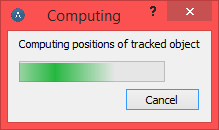
\includegraphics{png/progress_bar_infinite}
\caption{An infinite progress bar indicating that positions are being computed}
\label{fig:progress_bar_infinite}
\end{figure}
Since the computation is done in the VideoTracker module, the progress bar cannot be updated directly in the GUI module as it has no possibility to receive any information about completeness of the process, neither can user's cancellation be received when a process is carried out in a different module. Therefore, the progress bar is updated from the VideoTracker module while checking for a user cancellation. This is an exceptional situation where QT had to be used outside of the GUI module. When an output file is being created, a detailed progress bar indicates a percentage how many frames have already been processed.
\begin{figure}[!htbp]
\centering
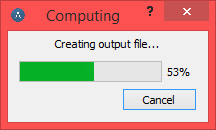
\includegraphics{png/progress_bar_detailed}
\caption{Detailed progress bar indicating that an output file is being created}
\label{fig:progress_bar_detailed}
\end{figure}

%%%%%%%%%%%%%%%%%%%%%%%%%%%%%%%%%%%%%%%%
\section{Showing a video}
\subsection{Drawing images}\label{subs:mat2qimage}
Showing a video is achieved by drawing images to a label. Since OpenCV uses its cv::Mat type for storing a video frame and QT uses QImage for holding an image, the former has to be converted to the latter so it can be displayed. The conversion takes place already in the VideoTracker. It is described in \autoref{subs:mat2qimage} as the GUI module does not use OpenCV.

\subsection{Playback speed}\label{subs:timer}
Video images are showed according to a timer for a smooth video playback. The timer is set to send a signal saying a new frame shall be displayed. The interval used for a correct video playback is computed from the video's fps. It would be convenient if a playback speed could be adjusted. This is accomplished by increasing and decreasing the timer's interval. However, the speed has its limit despite the application setting. The limitation is caused by high computation demands for reading, converting and displaying video frames. This means that there is a certain speed that cannot be exceeded and setting speed faster does not have any effect from this point. This could be improved by using OpenGL for images rendering. It would make showing a frame faster and the limit for a maximum speed would be increased, however, not removed.

\subsection{Original video}\label{subs:original_video}
The application always shows a video with all its objects. This is the way users can see how the output video would look like and any changes to objects are immediately reflected in displayed frames. In spite of this feature, users do not know how the original video looks like. Since added objects usually cover parts of the original video, it is not visible what exactly is covered. For this reason, an option for showing the original video beside the altered one was added. This option can be switched off due to the reason that it makes showing a frame slower and desired playback speed might not be reached. Moreover, users might want to see the altered video in details and are not interested in the original video. Switching the original video off adds more space for the altered one.

%%%%%%%%%%%%%%%%%%%%%%%%%%%%%%%%%%%%%%%%
\section{Object selection}\label{sec:selection}
\subsection{Selecting an area}
When a new object is being added for tracking, its area has to be selected. This is done by pressing a mouse button in a video frame at a position where the object begins, moving the cursor to the end of the object and releasing the button. The selection can be changed before it is confirmed the same way as the first selection was made. When users are expected to select an area, an initial selected rectangle is placed to the middle of the video frame to give a hint that selecting an area is expected. The selected area is displayed as a rectangle placed over the frame. This rectangle is drawn with QT since the object selection belongs to the GUI module and not to the VideoTracker that draws tracked objects with OpenCV. OpenCV is not used in the GUI module at all. 

\subsection{Converting mouse coordinates}
When a selection is being made, mouse coordinates are used for determining a position of the selected area. The displayed picture does not necessarily have the same size as the video frame because the size of the displayed picture depends on the size of the application window to which the video frame is resized. This is the reason why mouse coordinates need to be converted to the original video frame's size. An advantage of this approach is also that when a selection is being made and the application window is resized, the selection remains valid. Upon selection confirmation, these coordinates are sent to the VideoTracker to track the new object.

%%%%%%%%%%%%%%%%%%%%%%%%%%%%%%%%%%%%%%%%
\section{Tracked objects' settings}
\subsection{Key points}
Trajectory changes have to be easy to be made and maintained. For each object they are listed in a tab \keyName{Key points}. This list holds all information about points where a trajectory is changed. It includes also the object's first position and the last frame where it should occur. All these points have a context menu that gives options for its editing.
%\begin{figure}[H]
\begin{figure}[!htbp]
\centering
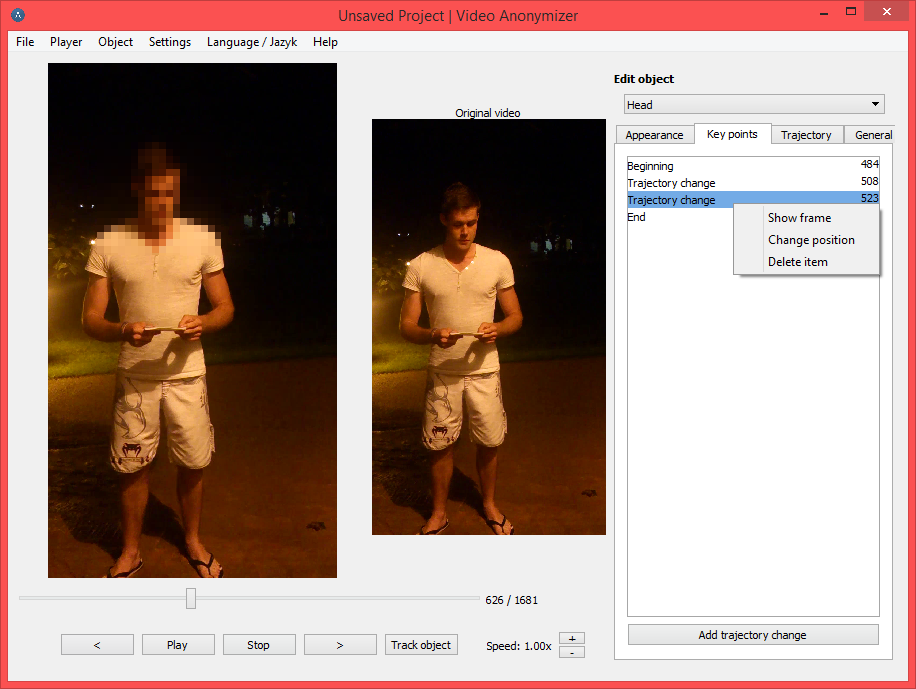
\includegraphics[width=\textwidth]{png/key_points}
\caption{Key points tab}
\label{fig:key_points}
\end{figure}

\subsection{Enabling settings}
The section for setting tracked objects shall be disabled until any object is added. This hints the user what the currently available possibilities are and avoids any distractions. The tracked objects section is disabled also when a certain operation is required (e.g. selecting a new object's area).

%%%%%%%%%%%%%%%%%%%%%%%%%%%%%%%%%%%%%%%%
\section{Object's appearance}
\subsection{Setting object's appearance}
When a tracked object is selected for editing, its current appearance settings shall be visible so it can be easily changed. Any change to its appearance is immediately reflected in the showed video frame provided the object is present in the frame.
\begin{figure}[!htbp]
\centering
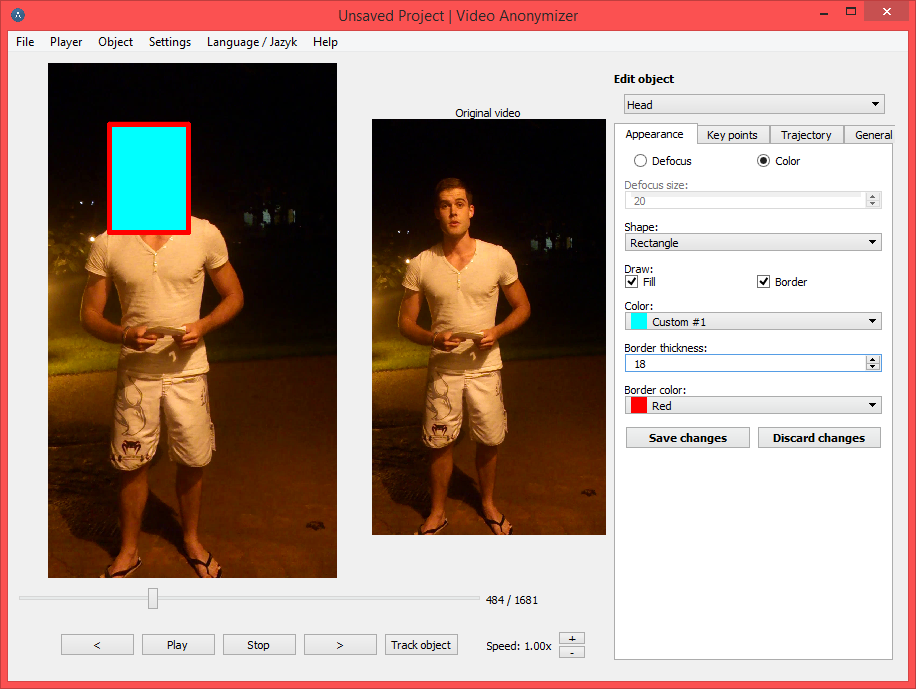
\includegraphics[width=\textwidth]{png/appearance_save}
\caption{Setting object's appearance}
\label{fig:appearance_save}
\end{figure}

\subsection{Discard / Save changes}
Even though appearance changes are immediately visible, they are not permanent until they are confirmed. When a change has been made, two buttons appear. One is for confirming the changes and the other one is for discarding them. When the confirmation button is clicked, the changes are accepted and they cannot be reverted. When discarding the changes, the previous appearance is restored. This is implemented by remembering the previous (original) appearance settings. For displaying changes immediately, they have to be sent to the VideoTracker to alter the currently displayed frame and send it back to the GUI module. If the changes are later confirmed, GUI module removes the saved previous settings and replaces them with the current ones as they are now the original settings. If changes are discarded, the VideoTracker is sent the previous (original) settings, the GUI module keeps the original settings and removes the altered ones.

\subsection{Ask to save changes}
The appearance changes need to be either saved or discarded before certain operations. These operations include editing another object, adding a new object, saving an output video and saving a project. This is required for users to know what exactly the object's state is so there is no misunderstanding. 
\begin{figure}[!htbp]
\centering
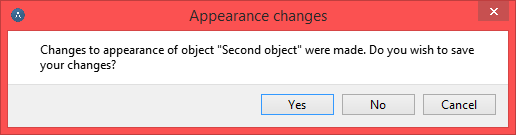
\includegraphics{png/save_appearance_changes}
\caption{An alert for saving appearance changes}
\label{fig:save_appearance_changes}
\end{figure}

\subsection{Custom colours}
Beside predefined colours, custom colours shall be enabled to be selected for filling an object or for its border. This is implemented by opening a colour picker that begins at the previously selected colour and enables picking any desired colour. The selected colour is saved upon confirmation and set as the current one. List of colours are the same for the object's filling as well as for its border. This means any added custom colour is added to both these combo boxes. When a project is saved, all the custom colours are included. See \autoref{sec:save_project}
%begin{figure}[H]
\begin{figure}[!htbp]
\centering
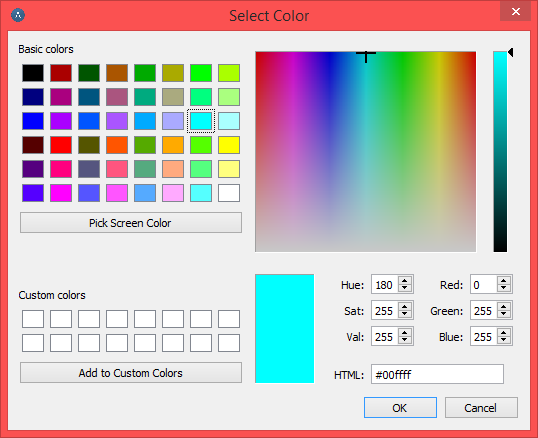
\includegraphics[scale=0.6]{png/colour_picker}
\caption{Colour picker for selecting a custom colour}
\label{fig:colour_picker}
\end{figure}

%%%%%%%%%%%%%%%%%%%%%%%%%%%%%%%%%%%%%%%%
\section{Displaying time positions or frame numbers}\label{sec:time_num}

\subsection{Frames identification}
Frames need to be somehow identified. Typical video players display the time position of a currently displayed frame and the total length of a video for an easier orientation in a video. This option has to be available in the application for an easier transition from a video player to the video anonymizer. However, this application is used for video editing and an option for precise frame identification is desired. Even though timestamps can be used for distinguishing frames, they are difficult to read by users. Frames' numbers (indices) are a better option as users exactly know what the number of the previous frame and the number of the next frame are. The total number of frames is also available (\autoref{sec:numframes}). Thus, the application can be set to either display time positions or frame numbers.

\subsection{Switching between types of identification}
Both types of identifications can be switched in the application settings. Beside displaying the identification beneath the showed video frame, it is present also in tabs Trajectory and Key points as well as in some application's alerts. This means when a type of identification is switched, all displayed values need to be changed. That is the reason why all the widgets include both kinds of information while only one of them is displayed. When a change occurs, the displayed information is replaced by the hidden one.

%%%%%%%%%%%%%%%%%%%%%%%%%%%%%%%%%%%%%%%%
\section{Saving a project}\label{sec:save_project}
\subsection{Project or video file}
The application enables creating an output video file that consists of an input video file and objects that were added. Even when the output video file is mostly the desired product of the application, it does not enable further editing once the application is closed. Therefore, there needs to be an option to save the state of the application. This state shall include the opened video as well as all tracked objects and their settings. The state of the application is from now on referenced as a \newExpr{project}.

\subsection{Serialization}
For saving a project, serialization is used. Data shall be stored in JSON or XML format so information can be extracted even outside of the application. This is possible when using the \newExpr{cereal} library~\cite{cereal}. It enables serialization and deserialization of C++ data types while storing the data in JSON and XML. Both these options are implemented in the application so users can decide which is more convenient for them. Each class that would be serialized needs to specify what members shall be stored. These members are then loaded when deserializing while all other members have their default values.

\subsection{Stored data}
Data that are stored in a project include an input video path, custom colours and objects with their settings. Objects' trajectories are stored as well, however, sometimes not all the trajectory is then loaded. Each object consists of sections that are described in \autoref{subs:sections}. A~trajectory can be loaded only for sections where the trajectory is computed from the section's beginning to its end. A~reason for this is that the tracking algorithm is initialized at a key point (beginning of a section) and needs to be gradually fed with all frames till the end of the section. If only a part of the section's trajectory was computed, the tracking algorithm would not be able to continue from this point. To solve this issue, each object's trajectory is checked upon loading a project and all computed positions of the last processed section are erased provided the section was not processed till its last frame.

\subsection{Asking to save a project}
Users can save and load a project whenever they like. In spite of that, they may forget about that when a project is being closed. That is the reason why they are reminded when closing the application or opening a new project if they wish to save the current project. However, they are reminded only if a project was changed from its last saving. 

%%%%%%%%%%%%%%%%%%%%%%%%%%%%%%%%%%%%%%%%
\section{Multilanguage support}
\subsection{Translation}
The application shall support two languages; Czech and English. This means a multilanguage support needs to be implemented. QT provides a possibility of translating an application by marking all the text that shall be translated. This text is extracted by a QT tool \newExpr{lupdate}. An output of lupdate is an XML file that holds original text strings together with their locations and a place for adding their translated equivalents. After all translated strings are added, QT tool \newExpr{lrelease} is used for creating a language file that is later attached to the application.

\subsection{Setting a language}\label{setting_language}
Language of the interface is at first chosen by environment's locale. Since only two language versions are available (Czech and English), the English version is set whenever the environment's locale is not Czech. The language can be changed explicitly, however, the change will take effect only after restarting the application. The reason is that the graphical user interface needs to be reloaded and so do all widgets added to the interface. For some widgets there are known issues of incorrect behaviour with changing the interface's language without restarting the application. The language choice is stored in settings that is described in \autoref{sec:settings}. Thus, it is always used when the application is run.

%%%%%%%%%%%%%%%%%%%%%%%%%%%%%%%%%%%%%%%%
\section{Settings}\label{sec:settings}
\subsection{Options of the interface}
Users shall be enabled to set the interface to suit their needs. Beside setting a language (\autoref{setting_language}), there are other options they can change. They can set if an original video is displayed (\autoref{subs:original_video}) and whether frame numbers or time values are used for determining positions in a video. (\autoref{sec:time_num}).

\subsection{Remembering settings}
Settings shall be saved so that it is loaded when the application is run the next time. Otherwise, users would need to change settings of the application every time the application is run. Beside explicit settings, some other information is saved as well. It is a path to the folder from which the last video was opened or to which the last video was saved. Thus, when running the application and opening a video, the default path is set to the previous one. Also an option whether to save a project in XML or in JSON is remembered. The same applies for loading a project.


%%%%%%%%%%%%%%%%%%%%%%%%%%%%%%%%%%%%%%%%
\section{User-friendliness}
\subsection{Ease of use}
Even when an application has lots of features, they might be difficult to find and use if they are not easily accessible or if it is not clear what their purpose is. This is the reason why the application is equipped with an application menu, tooltips, keyboard shortcuts and an application help. All these elements should make working with the application easier, especially when using it for the first time.

\subsection{Help}\label{subs:help}
The application has to be equipped with a documentation that helps a user when needed. QT offers a QT Help Framework that works with a help documentation written in HTML. After creating configuration files that describe the help structure that includes HTML help documentations, a QT help file can be generated. This file includes compressed help files as well as their structure and keywords. The application loads this file and displays the help right in the application when asked~\cite{walletfox_help}
\begin{figure}[!htbp]
%\begin{figure}[H]
\centering
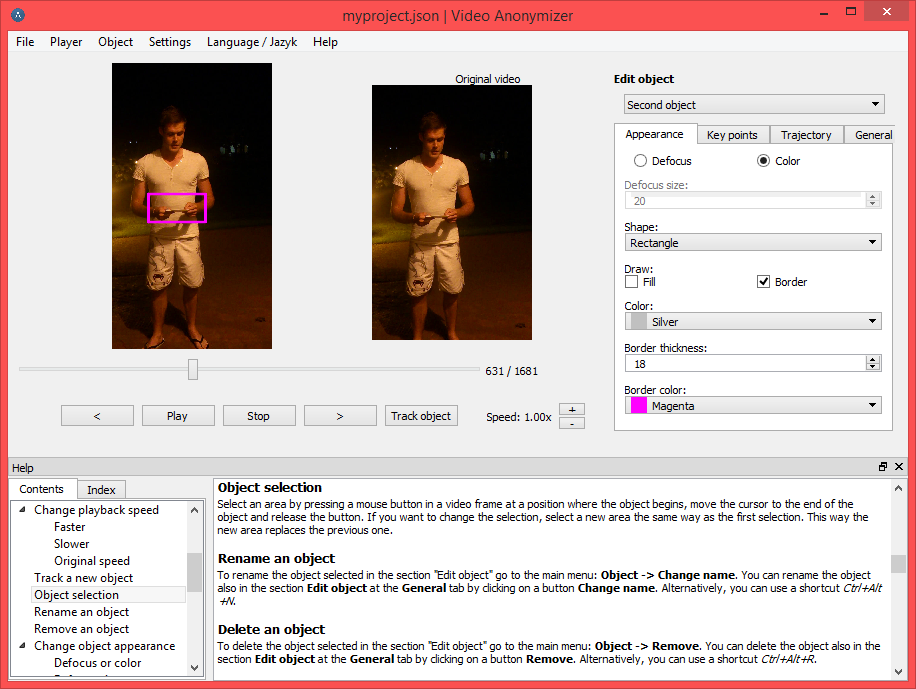
\includegraphics[width=\textwidth]{png/help}
\caption{Help displayed in the application}
\label{fig:help}
\end{figure}
The help in the application can be searched by its content as well as by its keywords.

\subsection{Menu}
The main application menu shall include all important options and settings even if those options are accessible from another place in the application. The reason being that it is easier to search the menu for a certain option than searching all the application. The main application menu is divided into sections that make searching the application menu easier. Options that are not accessible in the current application state are disabled so that users are always aware what options they currently have. For example, after running the application, the only available options are to open a video and to open a project. This is the way users are not distracted by other options since they cannot use them and a video or a project opening is needed for further work. Options that are present also outside the application menu are always in the same state as their application menu's equivalents.

\subsection{Tooltips}
Tooltips help understanding what a certain option is used for. When a mouse is hovered above a mouse widget, a bubble with a short description appears to tell a user what this widget does. It shall give a hint, not explain the widget's behaviour in details. More information about application options are available in the application's help described in \autoref{subs:help}.

\subsection{Keyboard shortcuts}
Options that are expected to be used the most were assigned keyboard shortcuts. This should enable controlling the application much faster for users who use it regularly. Keyboard shortcuts are mentioned in the application menu as well as in the application help.

%%%%%%%%%%%%%%%%%%%%%%%%%%%%%%%%%%%%%%%%%%%%%%%%%%%%%%%%%%%%%%%%%%%%%%%%%%%%%%%%
\chapter{Usability testing}\label{ch:testing}
\section{Performed tests}
The created application was tested by users to find out how user-friendly the graphical user interface is. The usability testing~\cite{usability_handbook} was performed by giving users a basic information about the application together with steps that users shall carry out while measuring the time it took them to complete each of the steps. Beside measuring time intervals, users were observed when working with the application and they were also asked for a feedback. Users were also instructed to search the user's guide for a certain information. Testing was performed by 11 participants with various levels of computer literacy. Participants were divided into two groups by the language version they used; Czech and English. There were no differences between results of testing Czech and English graphical user interfaces with user's guides in respective languages. Operating systems used for testing were Microsoft Windows 7, Microsoft Windows 8.1 and Fedora 21.

%%%%%%%%%%%%%%%%%%%%%%%%%%%%%%%%%%%%%%%%
\section{Results}
Results of the testing are very pleasing. Each step took users in average just a couple of seconds to be complete. Suggested improvements include placing a button for a trajectory correction among video player's controls and adding a possibility to correct the trajectory right in the list of trajectory items under the tab \newExpr{Trajectory}. An observed issue was that users were not certain what they can find under the \newExpr{Key points} tab and under the \newExpr{Trajectory} tab. As concerns the user's guide, users had no troubles finding and using it. All users agreed on the fact that the user's guide is comprehensive and easy to use when needed. 

%%%%%%%%%%%%%%%%%%%%%%%%%%%%%%%%%%%%%%%%%%%%%%%%%%%%%%%%%%%%%%%%%%%%%%%%%%%%%%%%
\chapter{Conclusion}
In this bachelor's project, I have developed an application for tracking and anonymizing objects in videos, called Video Anonymizer. This thesis describes its design and implementation. The application was developed as a part of a project \newExpr{Tools and Methods for Video and Image Processing for the Fight against Terrorism}\footnote{\url{http://www.fit.vutbr.cz/research/grants/index.php.en?id=498}}.

Firstly, I created a media player with an ability to jump to any desired frame (\autoref{ch:ffmpegplayer}). This ability raised issues of video compression and frames seeking that had to be solved. These issues are displayed graphically in \autoref{sec:seeking}. The media player is used by the core of the application, a video tracker (\autoref{ch:videotracker}). I have developed the video tracker to contain all the logic for operating the media player, tracking objects and anonymizing them. For the application to be user-friendly, I have created a graphical user interface that controls the video tracker (\autoref{ch:gui}). The graphical user interface is based on a typical video player's appearance so that the transition from using a media player to using the Video Anonymizer was the easiest possible.

Usability testing of the final application revealed that the graphical user interface and the application's guide are easy to use even with no prior experience with the application (\autoref{ch:testing}). Each tested procedure took just a couple of seconds to be complete. The application works on various platforms. It was tested on Microsoft Windows 7, Microsoft Windows 8.1 and Fedora 21. 

Used particle tracking algorithm for objects tracking is a weak point of the application. It could be replaced by a different one that is more accurate as a part of further development. The current algorithm supports only a rectangle shape. This results in tracking a bigger area than it is needed because not all shapes are rectangles. If the algorithm supported precise object's definition, the results would improve. With a better algorithm, objects' selection would have to be updated in the graphical user interface as well. The selection is currently made by placing a rectangle over a video frame. A better option would be to enable users to select points that create a polygon. Other possible improvements include adding bookmarks with objects' key points to the player's position slider and using the OpenGL library for displaying a video so that the video could be played faster when desired. 

%=========================================================================
 % viz. obsah.tex

  % Pouzita literatura
  % ----------------------------------------------
%\ifczech
%  \bibliographystyle{czechiso}
%\else 
%  \bibliographystyle{plain}
  \bibliographystyle{unsrt}
%  \bibliographystyle{alpha}
%\fi
  \begin{flushleft}
  \bibliography{literatura} % viz. literatura.bib
  \end{flushleft}
  \appendix
  
  %\chapter{Obsah CD}
\chapter{Manual}
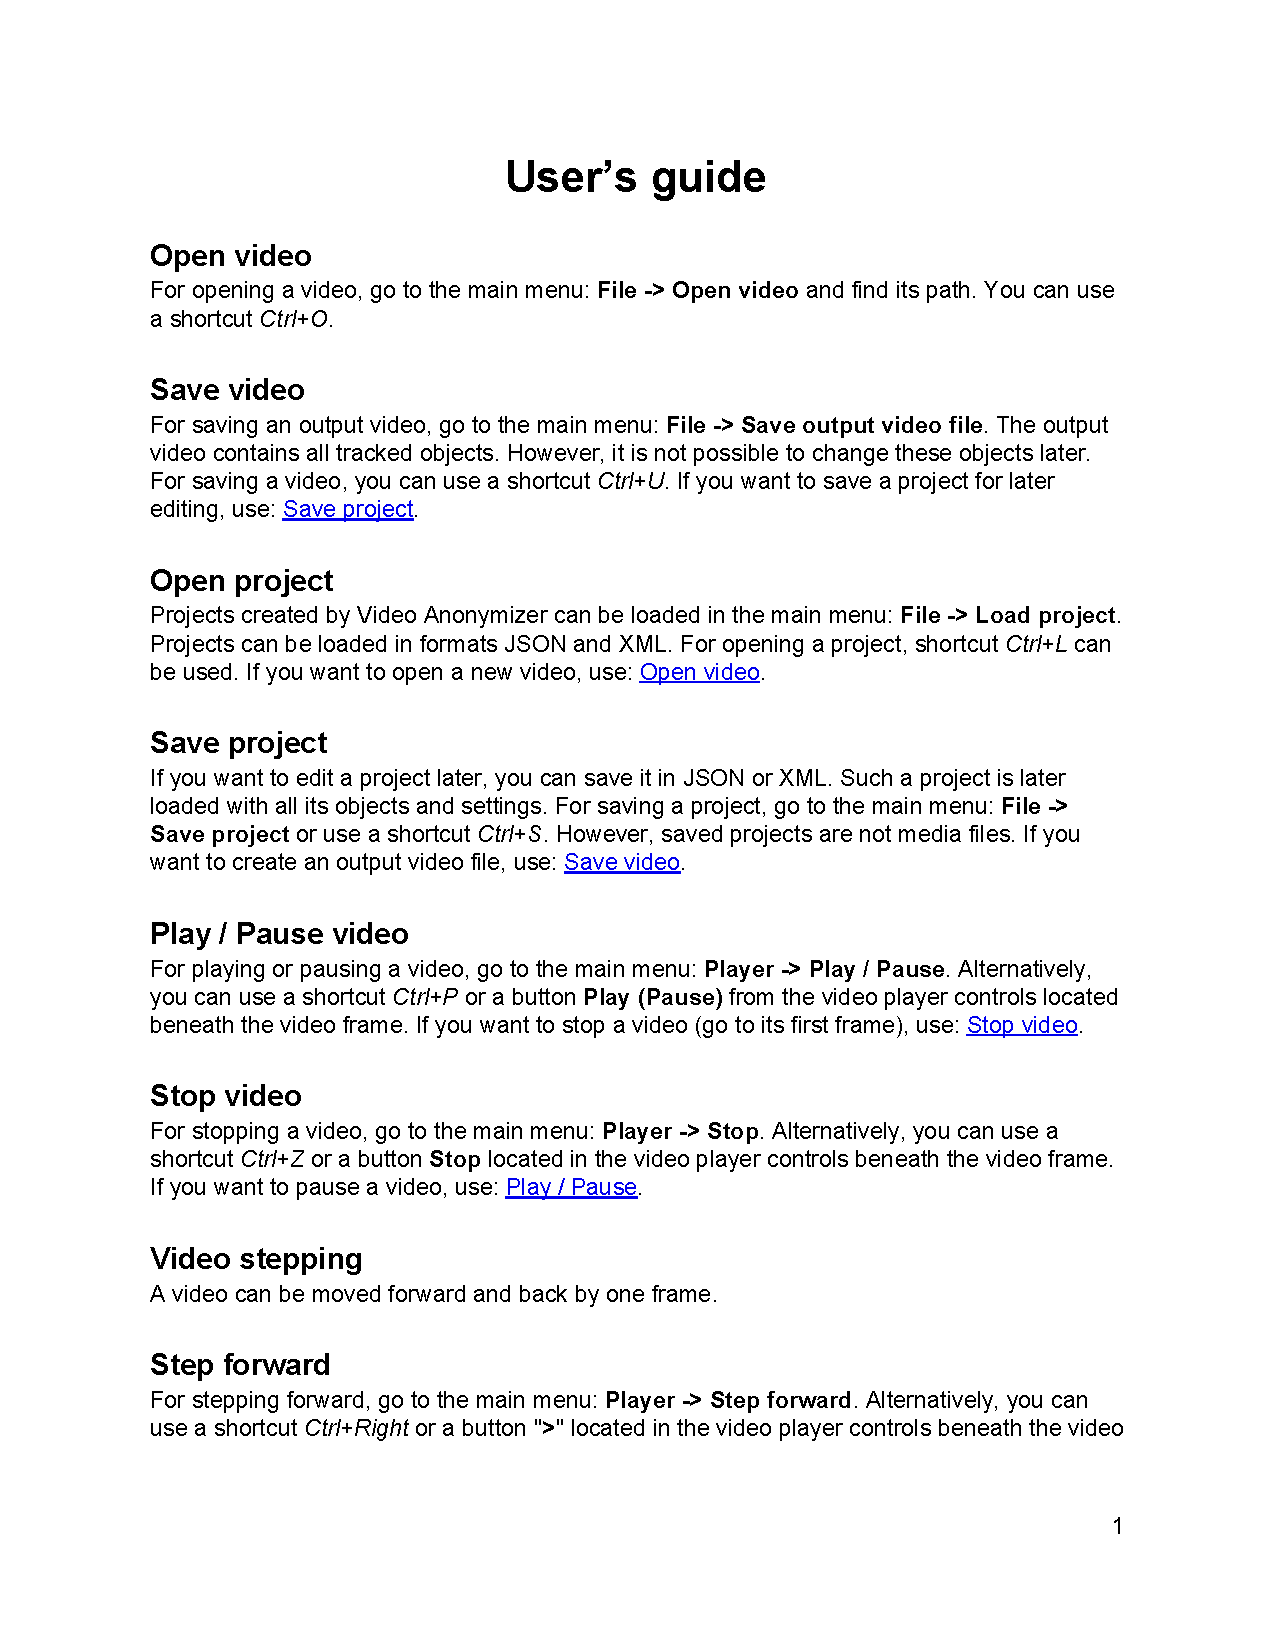
\includepdf[pages={1,2,3,4,5}]{append/manual.pdf}

\chapter{Usability testing - steps}
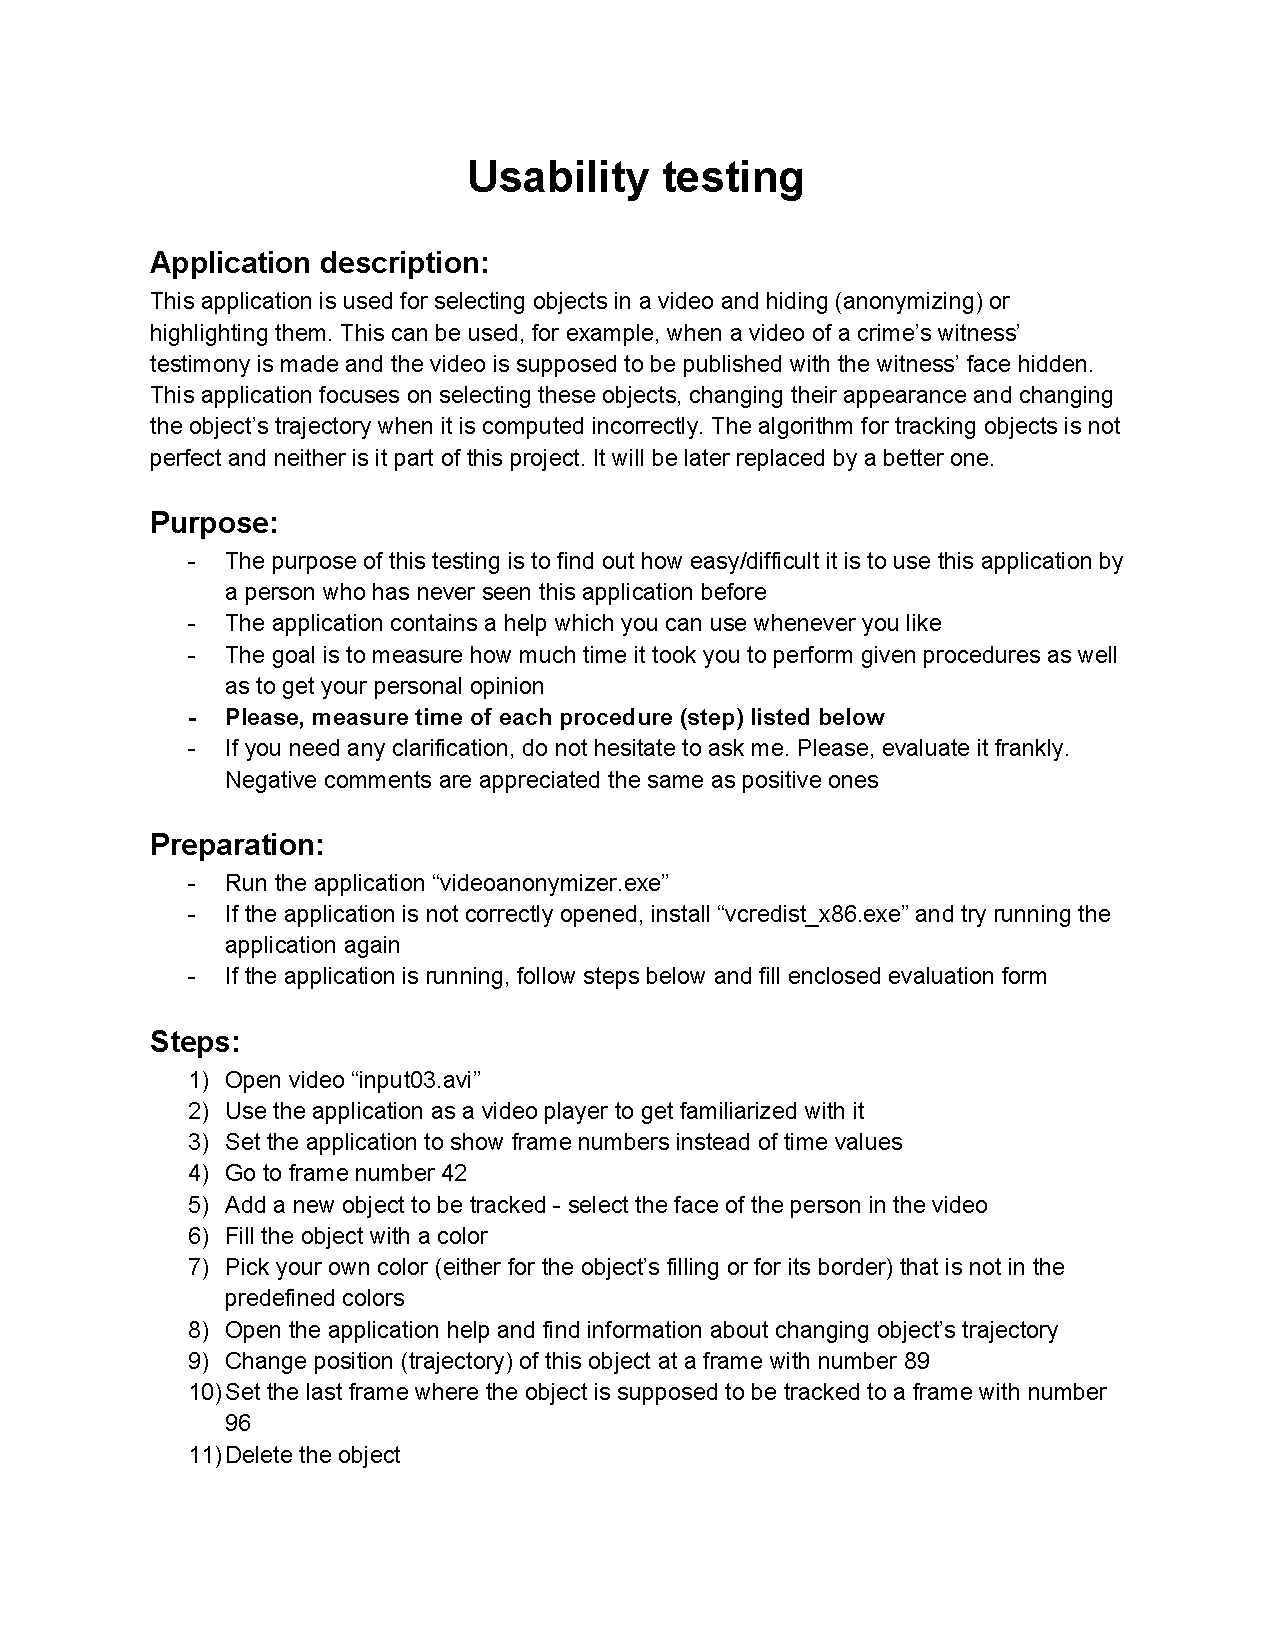
\includepdf[pages={1}]{append/usability_steps.pdf}
%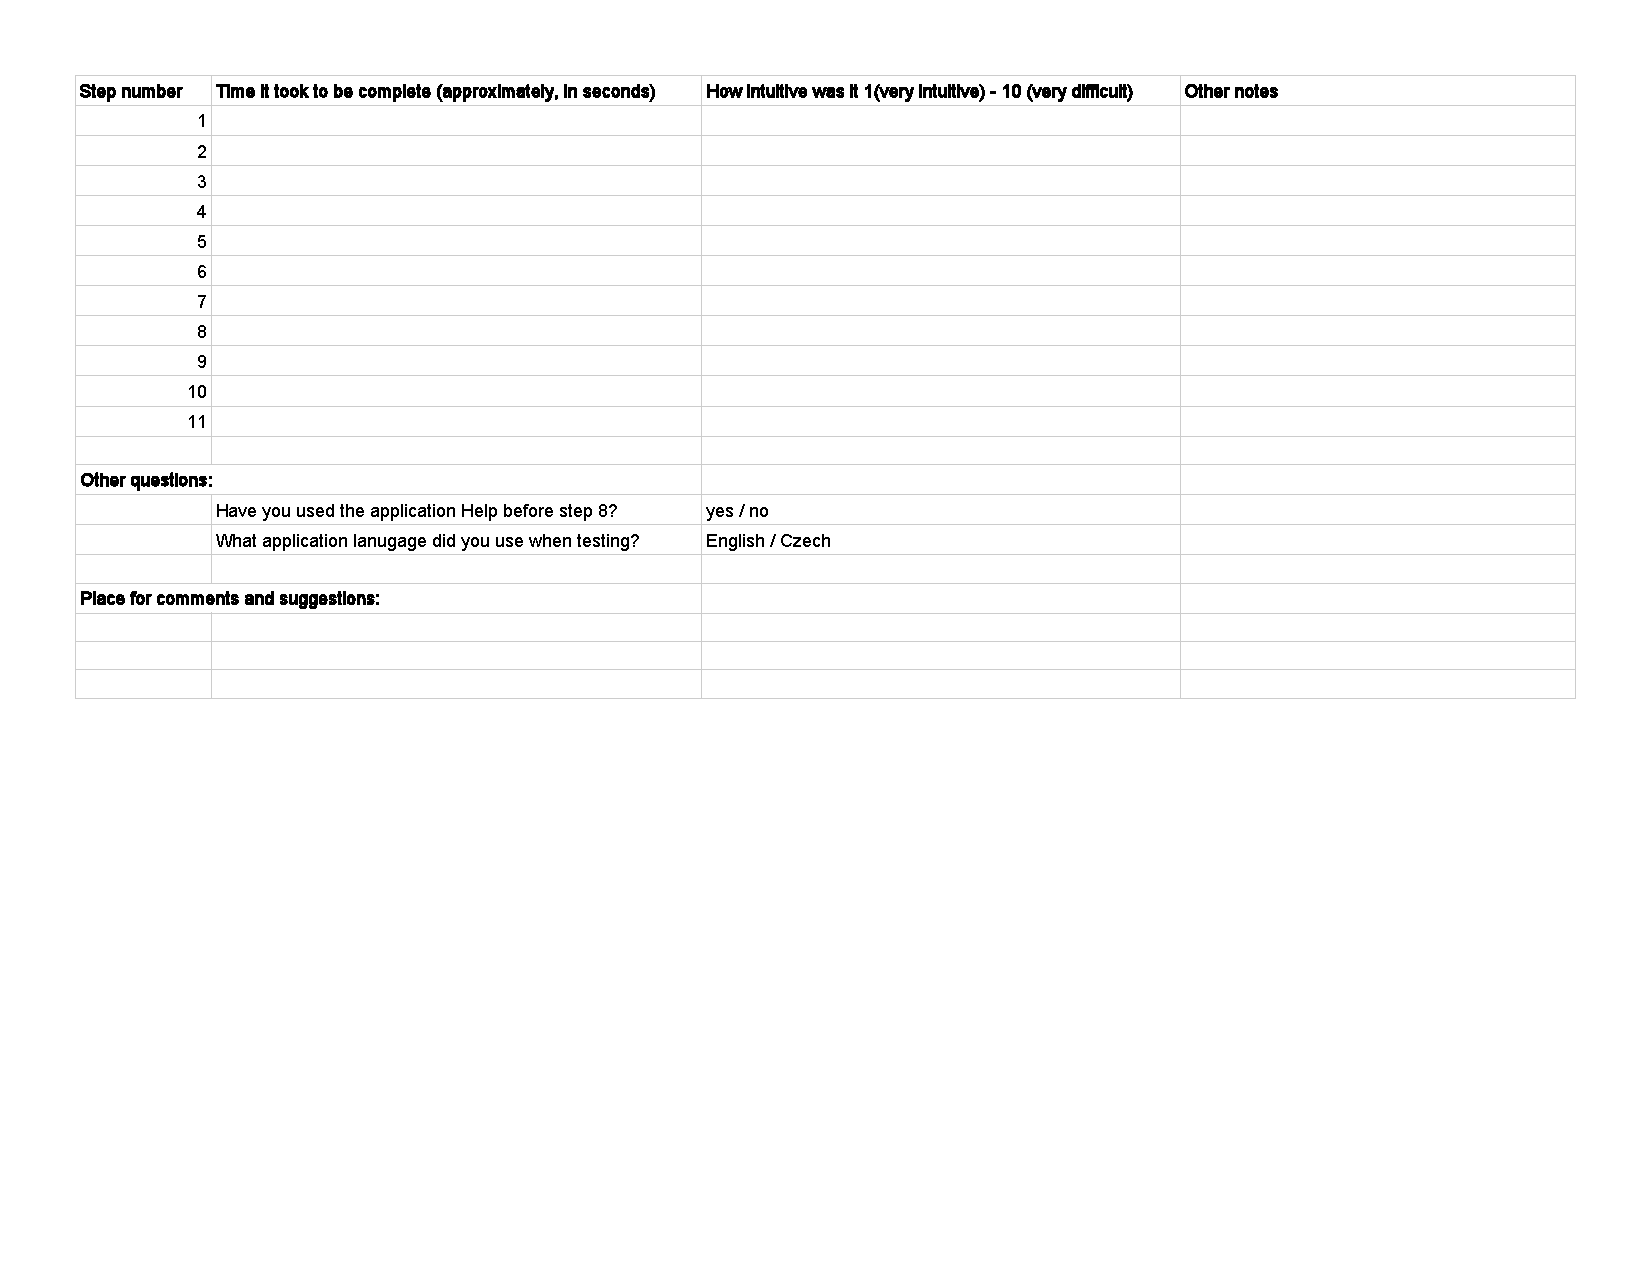
\includepdf[pages={1}]{append/usability_evaluation.pdf}

%\chapter{Konfigrační soubor}
%\chapter{RelaxNG Schéma konfiguračního soboru}
 % viz. prilohy.tex
\end{document}
